% Gravitational Waves

% Detector Configurations
    %% Interferometry with a Michelson configuration (MICH)
	%%% Contrast (Mode Matching Pt.1)
    %% Fabry-P\'erot Michelson (FPMI)
	%%% The Fabry-P\'erot Cavity
	    %%%% Arm Elongation
	    %%%% The Gaussian and Higher Order Modes (Pt. 2)
    %% Dual Recycled Fabry-P\'erot Michelson
	%%% Power Recycling
	%%% Signal Recycling

% ALIGO
    %% Thermodynamic Considerations
	%%% Adaptive Optics
	%%% Coating Thermal Noise

\section{Gravitational waves}
``Space-time tells mass how to move; mass tells space-time how to curve" can provide a concise and sufficient summarization of Einstein's theory of general relativity (GR). While providing the most complete theory of gravity to date, GR provides tools that allow considerations of high energy astrophyical phenomena (highly massive binary coalescences, spherically assymetric compact objects, etc.) whose fractional mass/energy output generate distortions in space-time known as gravitational waves (GW).
This is represented as a perturbation ($|h_{\mu \nu}|<<1$) in the Minkowski metric tensor defining a local linearized space-time:
\\
$$g_{\mu \nu} = \eta_{\mu \nu} + h_{\mu \nu}$$
\\
The wave-like behavior for $h_{\mu \nu}$ is realized after imposing the Lorentz gauge; producing 10 harmonic wave amplitudes from the Einstein field equations. Imposing a wave vector ($k_j$) onto one of three linearly independent spatial coordinates ($h^{ij}k_j$), the non-trivial amplitudes from the equations imply a transverse and traceless ($h^{i}_{i}$) gauge~\cite{misner:1973}:
\\
$$\nabla^2 h_{+} - \frac{1}{c^2} \frac{\partial}{\partial t} h_{+} = 0$$
$$\nabla^2 h_{\times} - \frac{1}{c^2} \frac{\partial}{\partial t} h_{\times} = 0$$
\\
In other words, there exists a wave solution with two separate transverse polarizations $h_{+}$ and $h_{\times}$ with a $45^{\circ}$ separation between them. 

\begin{figure}[H]
	\includegraphics[width=\textwidth]{INTRO/gw_particle_ring1.pdf}
	\caption{A stop motion pictograph displaying the influence of a single gravitational wave period from the two polarizations on a ring of particles. The top row shows the influence of the `+' polarization while the bottom row demonstrates that of the `$\times$' polariztion}	
	\label{fig:gwpolarizations}
\end{figure}

When measured and analyzed, these waves allow astronomers to extract novel information from their progenitors through the testing of various hypotheses pertinant to the violent dynamics of these systems. On September 14th, 2015 the Laser Interferometric Gravitational Wave Observatories made the first direct gravitational wave detection from a pair of coalescing black holes 1.3 billion light years away, and since then other gravitational wave detectors (i.e. Virgo, KAGRA) have joined the search; continuing the search for novel events. The current GW detector network has developed a track record with an ever increasing list and rate of detections including the first multimessenger event and a suprising population of compact binary coalescences ~\cite{gw170817, nitz:2023}. 

A more experienced reader may be familiar with the following primer to gravitional wave instrumentation, but it is all done with the hope of providing context of novel contributions within the body of this work while also demonstrating reverence to those whose work prior made this dissertation possible. 

\section{Detector configurations}\label{sec:detcon}
The current gravitational wave detector network primarily uses terrestrial bound Dual-Recycled Fabry-P\'erot Michelson interferometers; though to configure them into a state of observing, fundamental modes of operation are necessary to acquire first. A quick review of these modes provides some of the basic ``whats'' and ``hows'' of detector operation with the intention of developing a holistic view of the LIGO detection schema especially as it pertains to the studies to be discussed. Most introductory detector configuration discussions start with the Michelson interferometer and end at the dual-recycled Fabry-P\'erot Michelson interferometer; this section follows in kind. Alongside the discussion are citations providing exceptional alternative and more detailed explanations of topics discussed.

\subsection{Interferometry with a Michelson configuration}
The Michelson interferometric detection schema (aka ``The Michelson''), used by Michelson and Morley to test the existence of luminiferous aether, demonstrates inherent potential for measuring gravitational wave amplitudes generated by time varying quadrapole moments with high energy astrophysical progenitors; making it a prime candidate as a gravitational wave detector / observatory. The interferometry begins with a beam of coherent laser light split at a 50/50 beamsplitter ($\mathrm{BS}$) along two perpendicular beam paths with respective lengths $L_x$ and $L_y$, set by highly reflective end mirrors ($\mathrm{ETMX}$, $\mathrm{ETMY}$). Upon arrival at the length terminating mirrors, the respective beams are back-reflected towards the beam splitter where they are made to interfere. The fringe power from this interference is measured at the anti-symmetric port photodiode: 

\begin{equation}\label{fig:pmichas}
	P_\mathrm{out} = \frac{P_\mathrm{in}}{2} \bigg[1+\mathrm{cos}\Big(\frac{4\pi}{\lambda} (L_x - L_y)\Big) \bigg]
\end{equation}

The Michelson detects microsocopic differential length changes on the order of a fractional wavelength of the light used and are more aptly discussed as differential phase ($\Delta \phi(t)$) between the returning perpendicular phasefronts ($\phi_x(t)$, $\phi_y(t)$). Understanding this inherent method of detection, a time-varying metric perturbation ($h(t)$), like that generated from a gravitational wave, is tested on a Michelson interferometer with a nominal arm length of L and a laser with optical angular frequency of $\Omega$:

\begin{equation}
\Delta \phi(t) = \phi_x(t) - \phi_y(t) =  \int_{t-2L/c}^{t} \Omega \bigg[1 + \frac{1}{2}h(t)\bigg]dt - \int_{t-2L/c}^{t} \Omega \bigg[1 - \frac{1}{2}h(t)\bigg]dt 
\end{equation}

\noindent Evaluating the above as a function of frequency yields:

\begin{equation}\label{fig:michdelphi}
	\Delta \phi (\omega) = h_0\frac{2 L \Omega}{c}e^{-i L \omega / c} \frac{\mathrm{sin}(L \omega /c)}{L \omega /c} = h_0 \cdot H(\omega, \phi_0)
\end{equation}

With the wave amplitude $h_0$, angular frequency $\omega$, nominal interferometer arm length $L$, and speed of light $c$.
The differential phase \autoref{fig:michdelphi} combined with the power at the anti-symmetric port \autoref{fig:pmichas} provides a function of optical gain, dependent on frequency and a differential offset phase ($\phi_0$):

\begin{equation}
	\Delta P(\omega, \phi_0) = h_0 \frac{P_\mathrm{in}}{2} \Delta \phi (\omega) \cdot \mathrm{sin}(\phi_0)
\end{equation}

\begin{figure}[ht!]
	\begin{subcaptiongroup}
		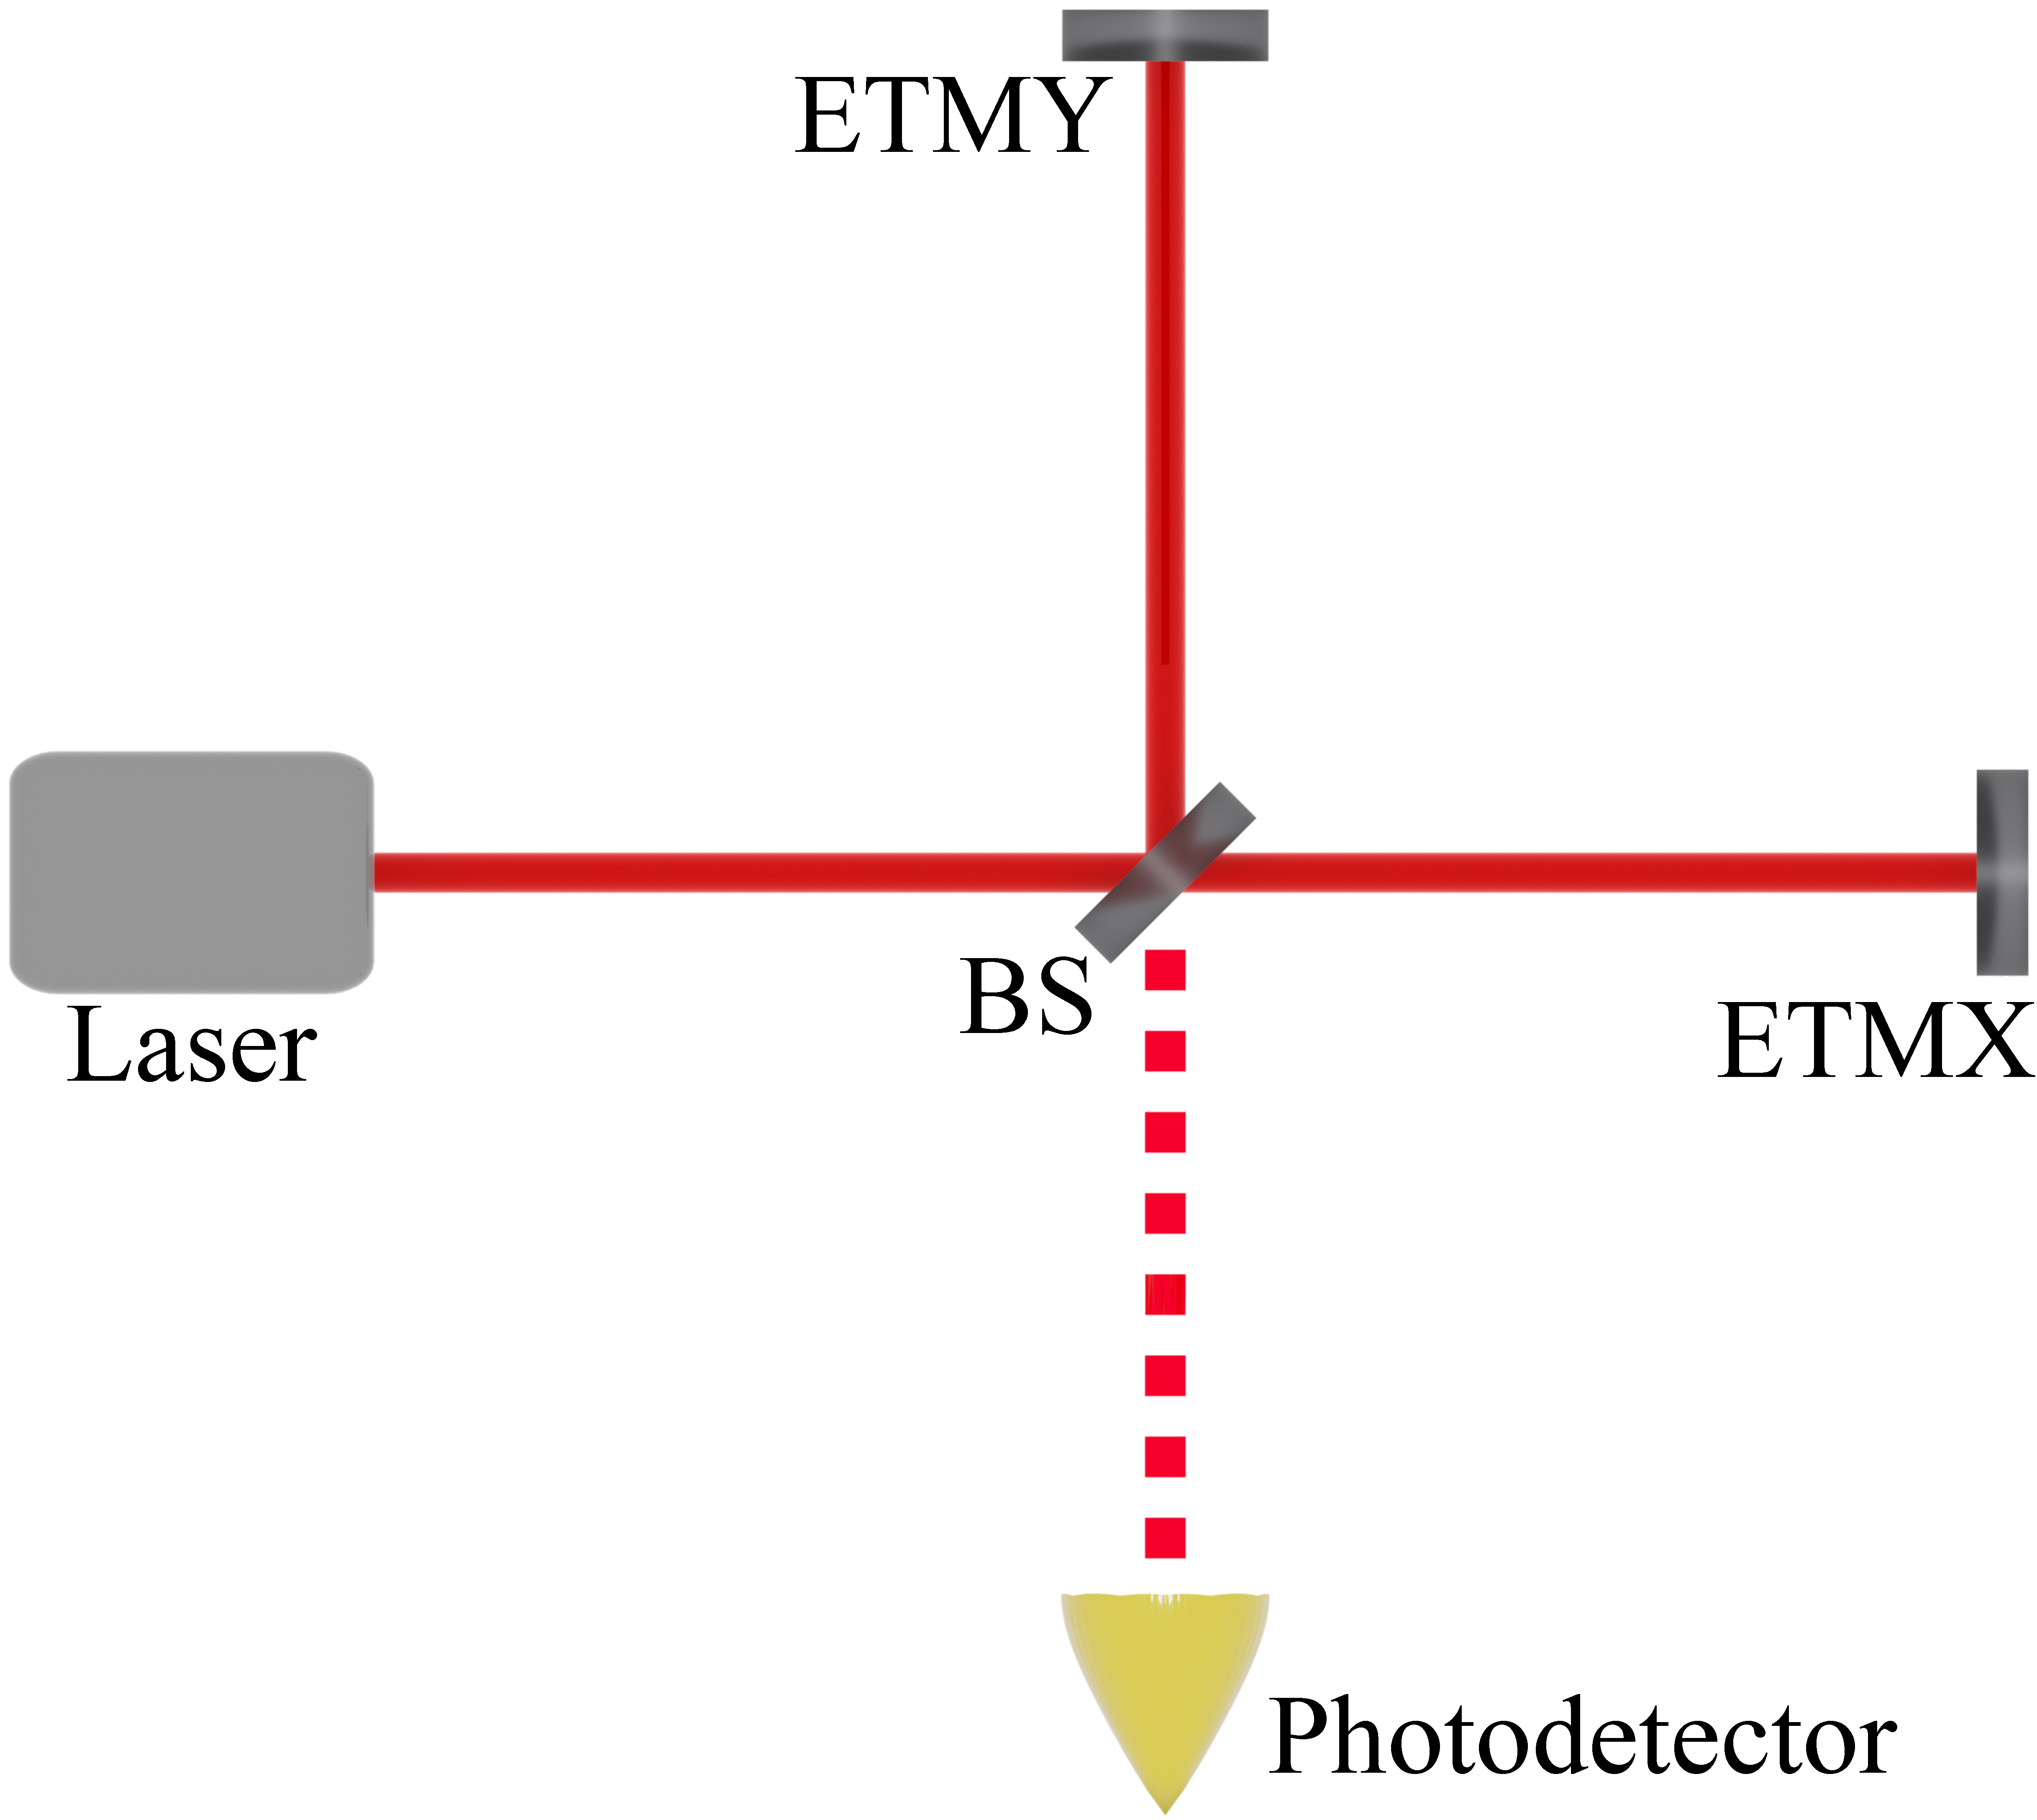
\includegraphics[width=.45\textwidth]{INTRO/mich_new.pdf}
		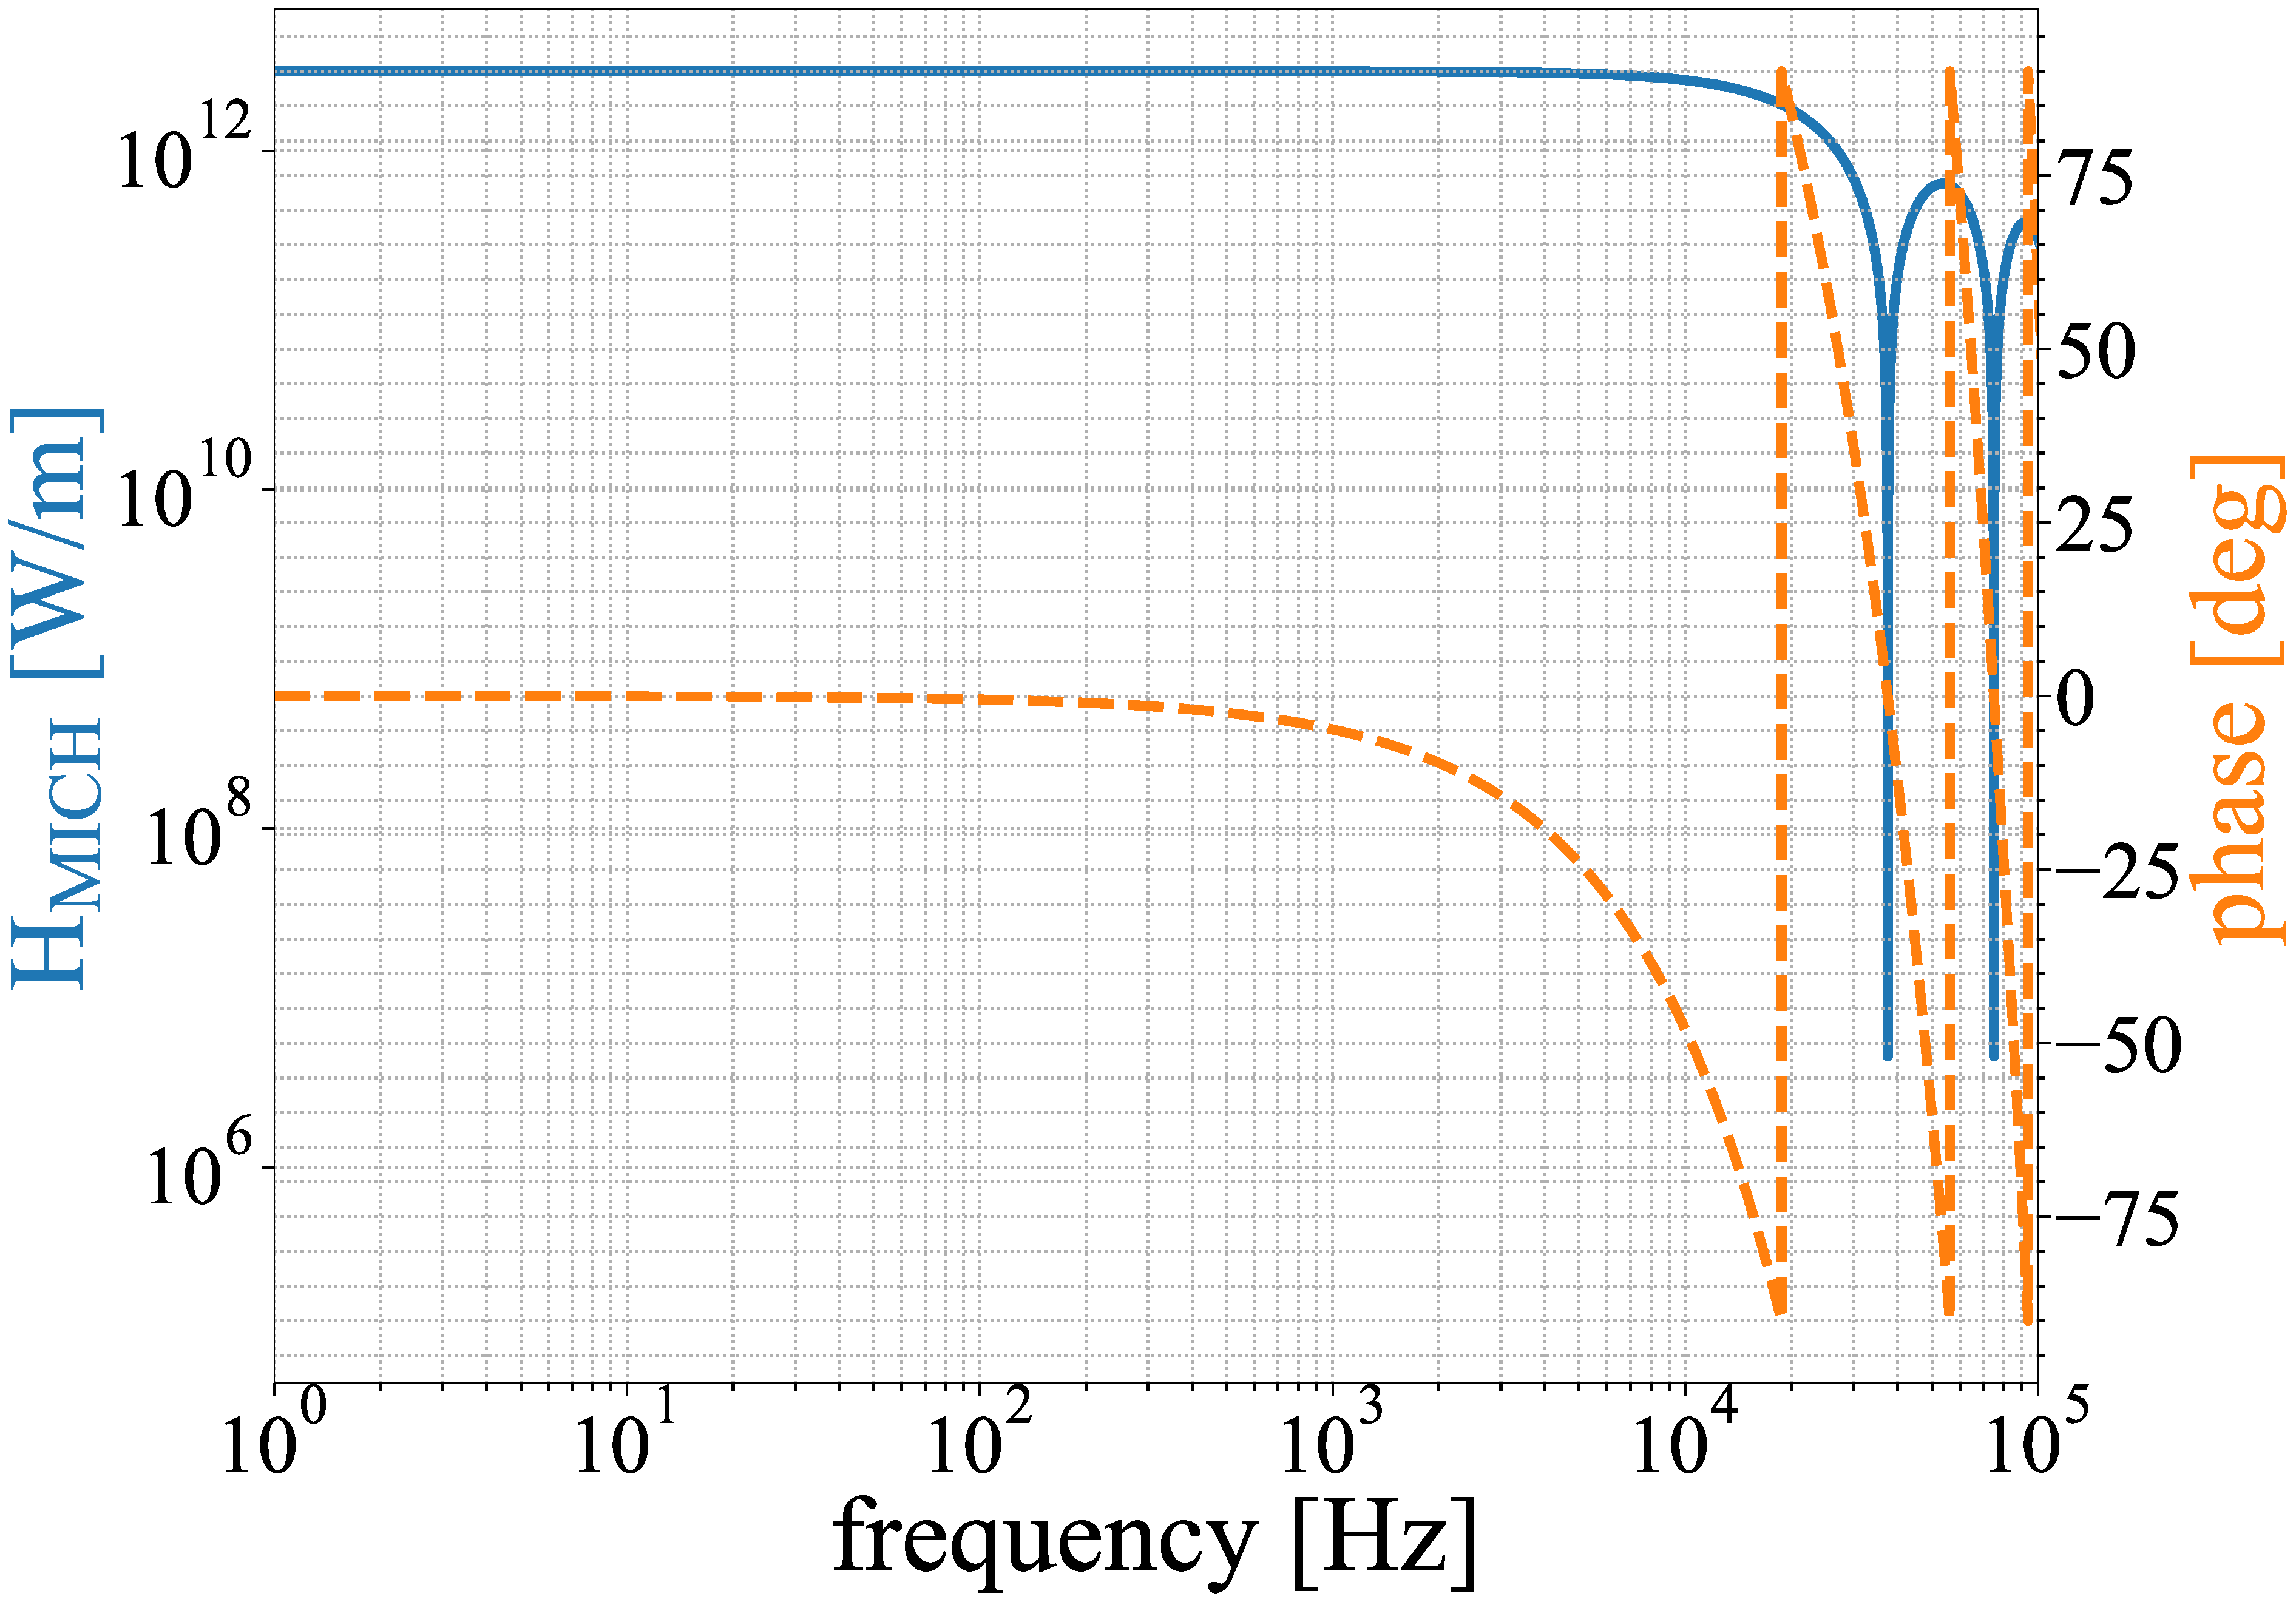
\includegraphics[width=.575\textwidth]{INTRO/mich_fr.pdf}
 	\end{subcaptiongroup}
  	\hfill
	\caption{[Left] A simplified schematic of a Michelson interferometer. [Right] The associated optical transfer function with $H(\omega, \pi/2)$ defining the optical gain of a Michelson interferometer with 4 km long arms and an input power of 25 [W]}
		\label{fig:mich}
\end{figure}
\FloatBarrier

Assuming a 4km arm configuration with 25 Watts input power as indicated in figure \autoref{fig:michdelphi} the differential arm response provides a reasonable optical gain with the notches coorelating to an integer number of gravitational wave half periods ($\mathrm{n}\lambda_{gw} / 2$) to the interferometer arm length in such a way that the response is null for cooresponding frequencies. Though with sights set on optimizing detection bandwidth for neutron star (NS) binaries @ 100 Hz, the basic Michelson optical gain remains insufficient, with enhancements required. This is better visualized by computing the shot noise limited Michelson sensitivity which does not reach he requirement to confirm a NS-NS coalescence ($\approx 10^{-21} \; [\frac{1}{\sqrt{\mathrm{Hz}}}]$) but an astonishing start nonetheless ~\cite{saulson:2017}.

\begin{figure}[H]
	\centering
	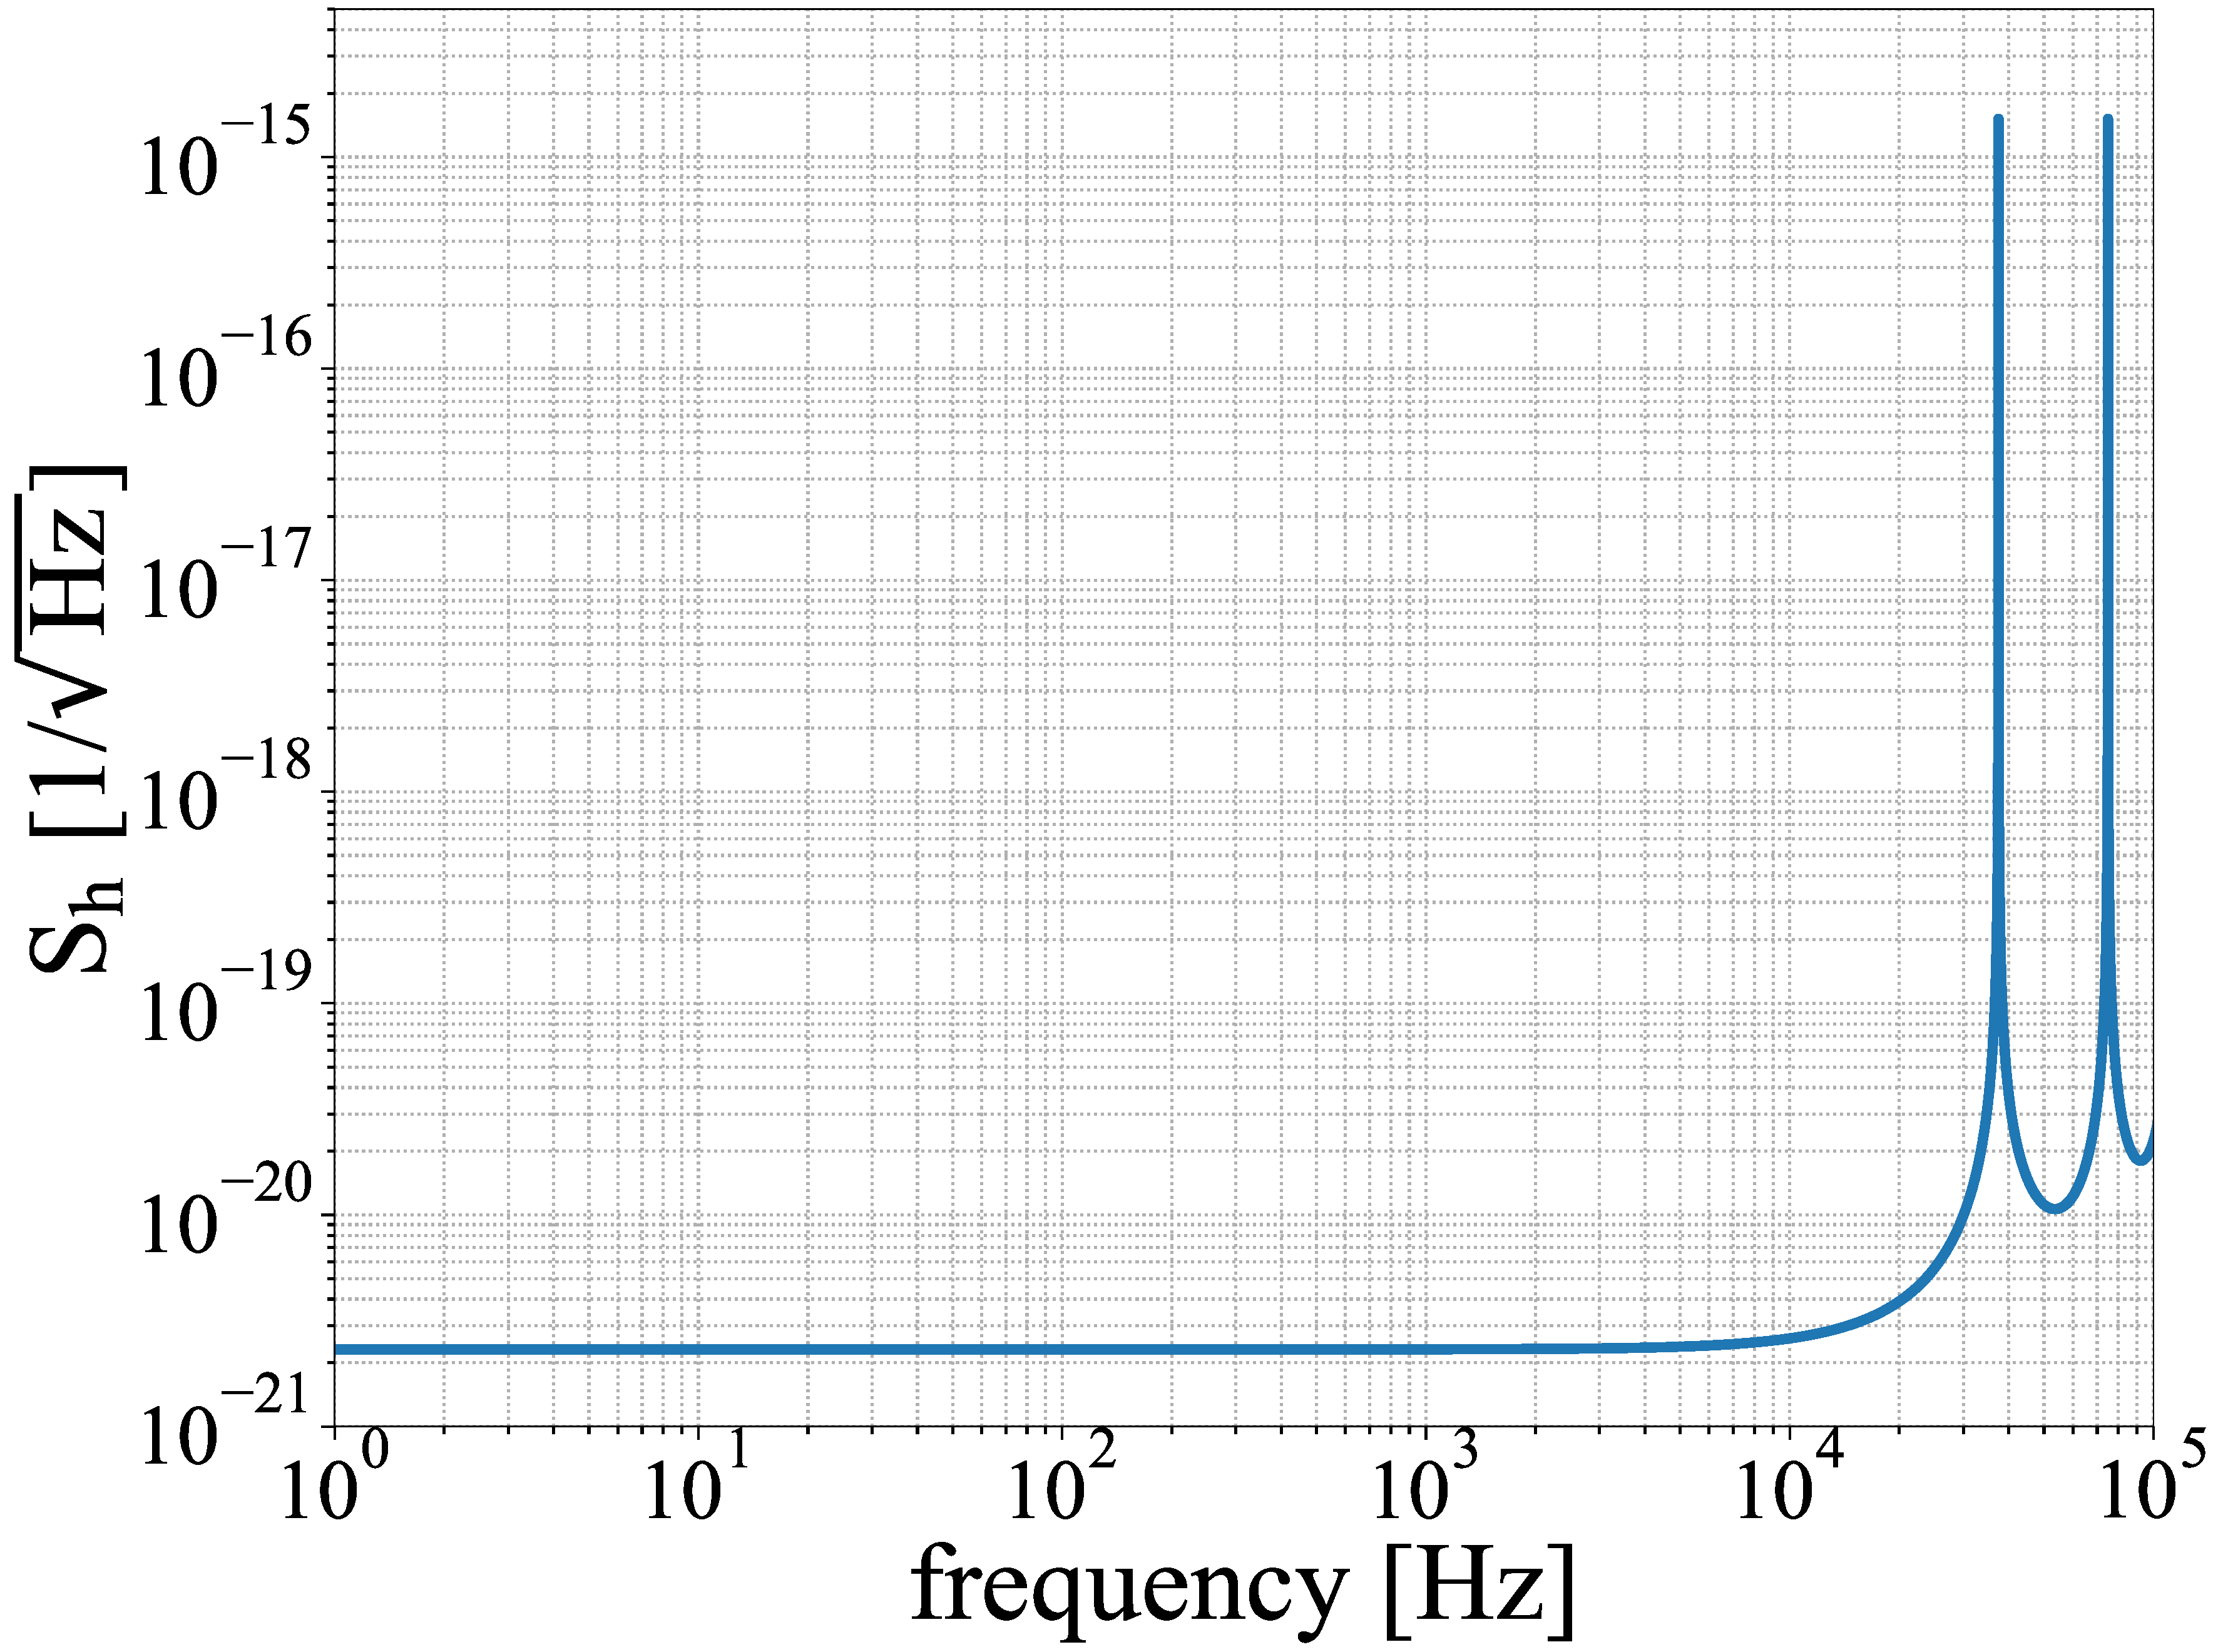
\includegraphics[width=\textwidth]{INTRO/mich_sensi.pdf}
	\caption{Shot noise limited sensitivity ($\sqrt{\hbar \Omega P_\mathrm{in}}$) of a Michelson with 4 km long arms and an input power of 25 [W]. Compared to the apriori estimate of $10^{-21} \; [\frac{1}{\sqrt{\mathrm{Hz}}}]$ the signal to noise (SNR) comes to be unity. The desired confidence is set at a much higher standard with more unquestionable measurements set at SNR = 5.}
	\label{fig:michsensitivity}
\end{figure}

\subsubsection{Contrast (Mode Matching Pt. 1)}
As presented, the functional behavior of the simple Michelson is to perform optical autocoorelation; though overly simplified depictions of interferometry suggest operation by periodic planar phasefronts and omit the full reality of Gaussian beam propogation. A standard laser carrier beam mode is represented by the Gaussian beam (TEM00 mode) with wavelength $\lambda$, and propogation axis ($z$):

\begin{equation}\label{eq:gaussianbeam}
E(r) = E_o \frac{\sqrt{[\lambda z_o] / \pi}}{W(z)}e^{-r^2 / W^2(z)} e^{-ikz - ik[r^2 / (2R(z))] + i \zeta(z)}
\end{equation}

Where $E_o$ is a complex field amplitude, $r^{2}/(2(R(z))$ defines transverse coordinates $r = \sqrt{x^{2} + y^{2}}$ on a hemisphere of uniform phase with a radius of curvature $R(z)$, $k$ is the wave number, $W(z)$ is the radius from the beam axis that contains $(1-1/e^2) \times 100 \%$ of the integrated beam power, and $\zeta$ is the Gouy phase ~\cite{salehteich:2007}. 

An important consideration to make for any sufficiently long arm length (like that used for LIGO), is avoiding significant power loss due to beam divergence for the designed Michelson arm length, sans sufficiently large core optics. LIGO and most other terrestrial GW detectors manage with curved end mirrors that match and focus the impinging hemispherical wavefronts; symmetrically back-propogate them in each arm to maintain optimal interference at the beamsplitter. Mode overlap $\eta$ provides a useful metric of this optimization: 

\begin{equation}\label{eq:modeoverlap}
	\eta = \bigg|\int E_x E_y dA \bigg|^{2} \bigg/ (P_x P_y) 
\end{equation}

Significant length offsets between the arms reduce the integrated phasefront overlap and contribute to sub-optimal interference of the beam mode wavefronts at the beamsplitter. And even without 2D beam profiles at the output, measuring the dark and bright fringe power on single element photodiodes and computing contrast a.k.a interferometer visibility ($\nu$) may do just as well without more involved beam mode analysis:

\begin{equation}\label{eq:contrast}
	\nu = \frac{P_\mathrm{max} - P_\mathrm{min}}{P_\mathrm{max} + P_\mathrm{min}}
\end{equation}

Operating on a scale from 0 to 1, $\nu \le 1$ can be an indication of : mode mismatch at the beam splitter and/or assymetrical optical loss. From a mode matching perspective $\nu = 1$ represents a mode overlap of $\eta = 100 \%$ (assuming no optical loss).  Though optical losses and aberrations are often asymetrically introduced between the orthogonal beam paths that often limit optimal interference and are indiscriminately accounted for in contrast measurements.  

\subsection{Fabry-P\'{e}rot Michelson (FPMI)}
At the time of the LIGO proposal, constraints (physical and financial) for terrestrial gravitational wave detectors required a compact solution for increasing length (L) of the Michelson arms so to increase the beam phasefront lifetime within the Michelson arms. Two proposed arm folding techniques were considered: the Herriot Delay Line and the Fabry-P\'{e}rot cavity, though the Fabry-P\'{e}rot cavity is currently the predominent choice.

\begin{figure}[ht!]
	\centering
	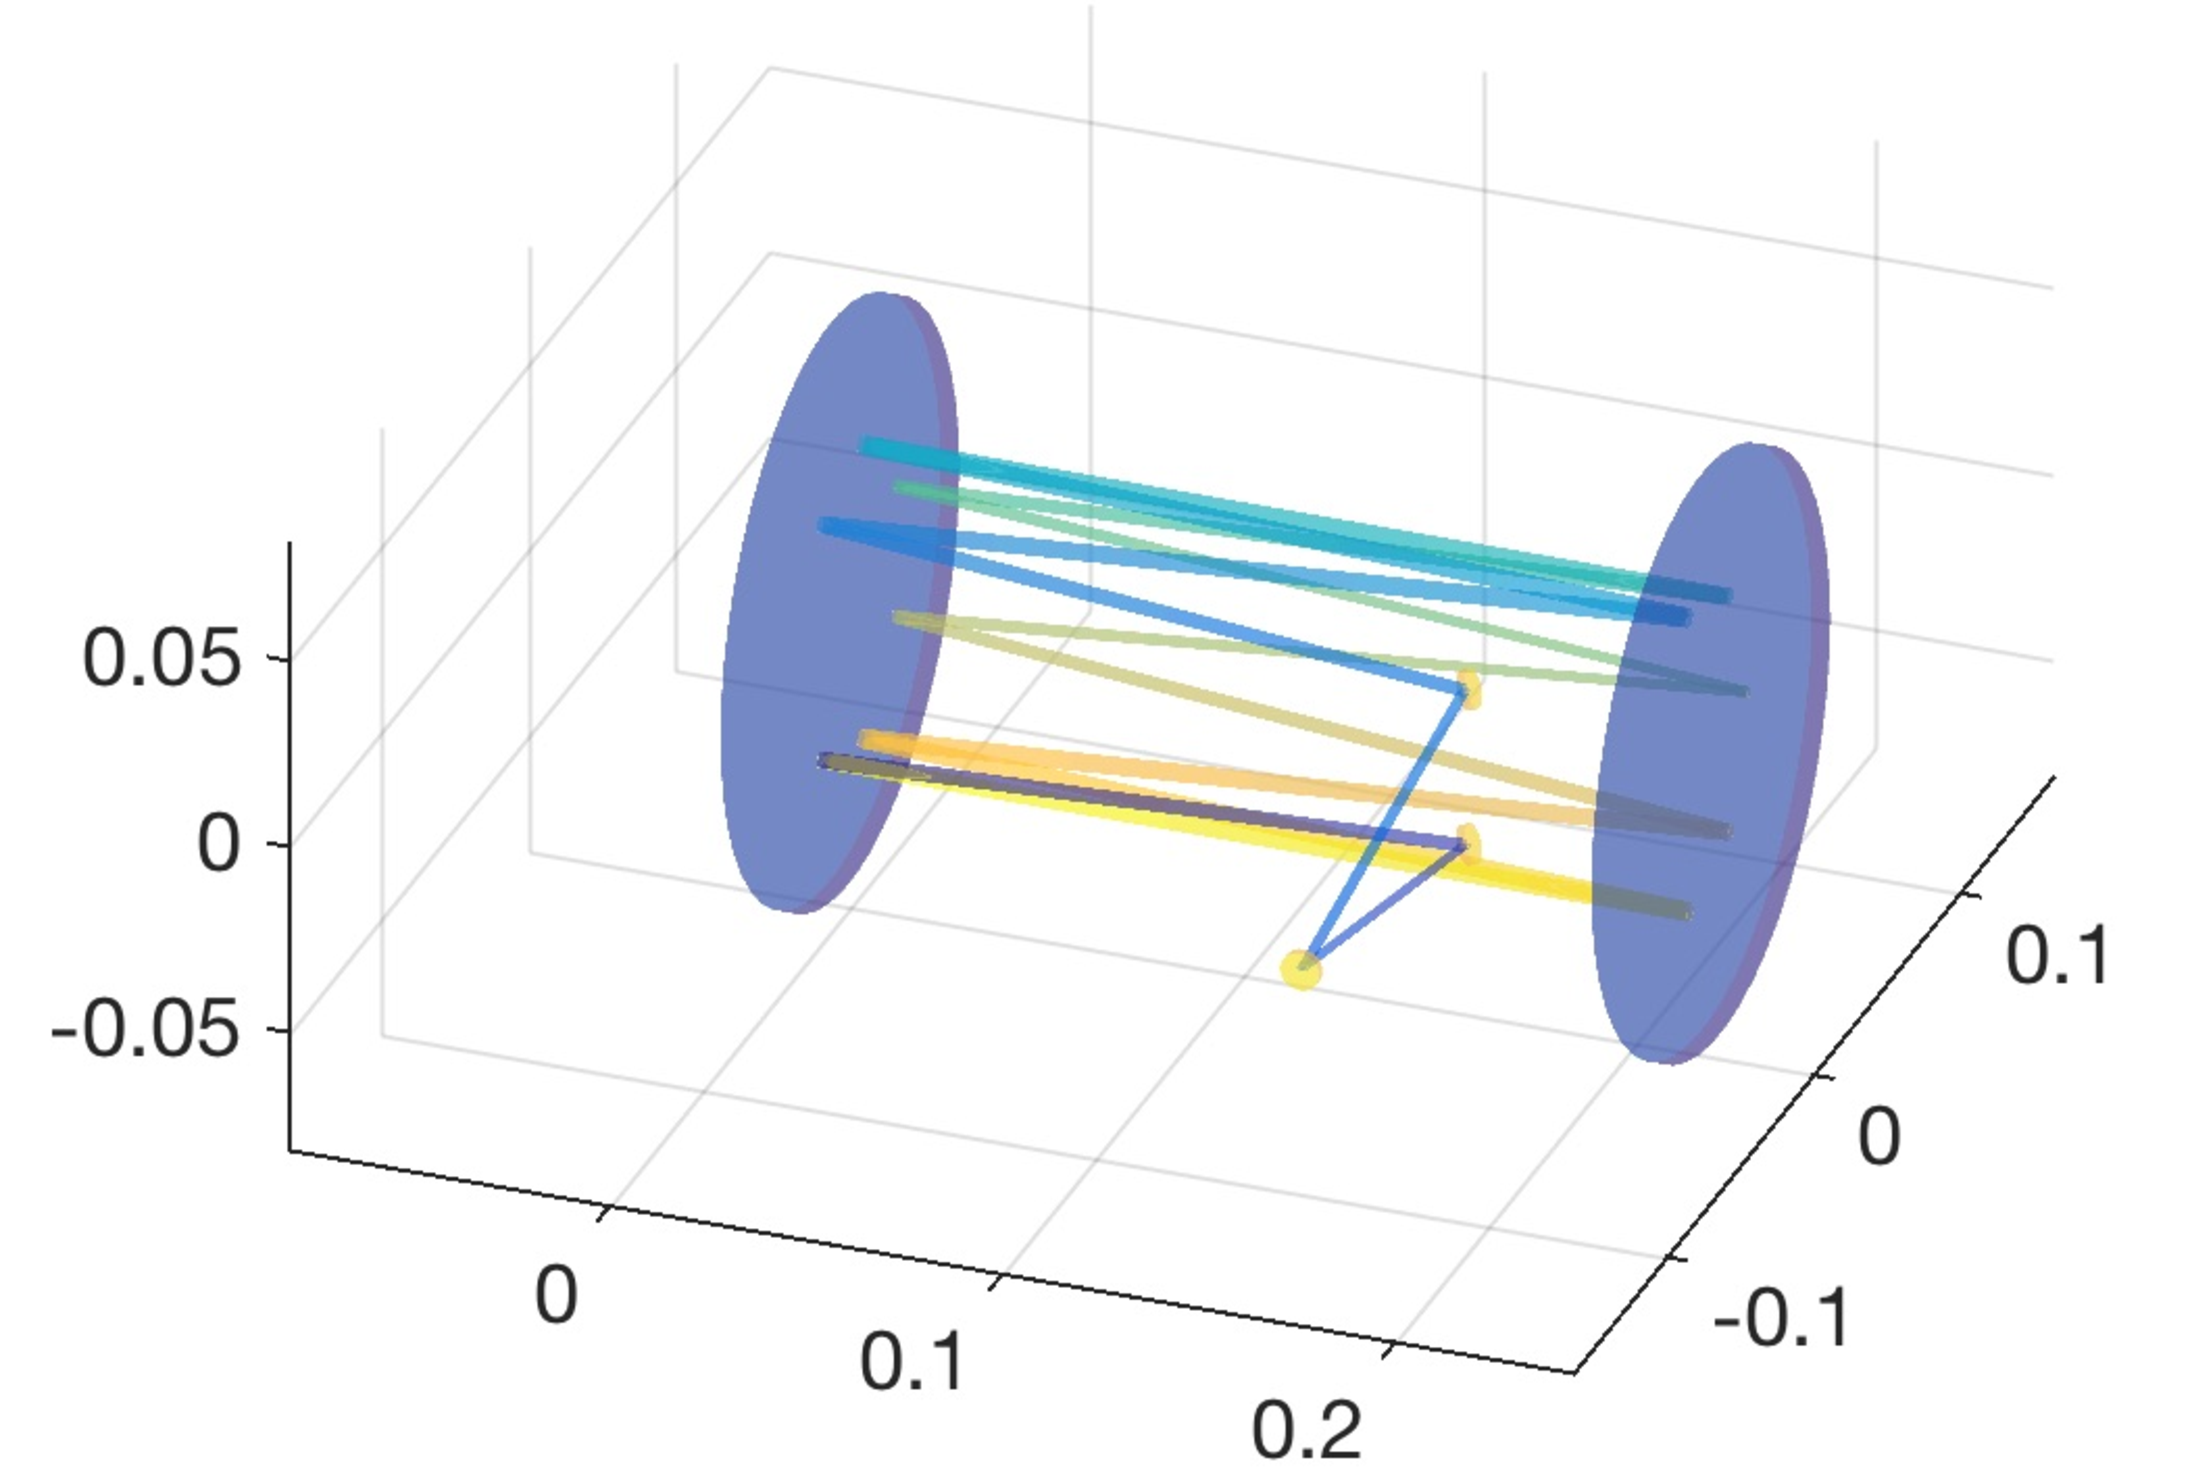
\includegraphics[width=\textwidth]{INTRO/HDL.pdf}
	\caption{A 12 bounce Herriot Delay Line with a small mirror input / output couplers inserted into the beam path.}
	\label{fig:hdlcav}
\end{figure}

\subsubsection{The Fabry-P\'{e}rot cavity}
\label{sec:FPC}
To inform of a folding mechanism, consider coherent light encountering an optical cavity with input and output mirror transmission and reflection coefficients of $t_1$, $r_1$ and $t_2$, $r_2$ respectively (assuming lossless mirrors $L_1 + L_2=0$).

\begin{figure}[h!]
	\centering
	\includegraphics[width=\textwidth]{INTRO/simple_fp.pdf}
	\caption{Figure of a Fabry Perot Cavity}
	\label{fig:fpcav}
\end{figure}

Light enters the cavity only after passing the input mirror with the trivial solution indicating a field amplitude reduction proportional to the mirror reflection coefficient. Though by tuning the length between the input and end mirrors to an integer multiple of the beam wavelength, circulating light coherently adds with the input, achieving resonance.  A cavity of length $L$, when configured, yields the following cavity reflection and transmission coefficients: 

\iffalse that the input and circulating that the photons belonging to a particular phasefront can be experimentally tracked, and lucky for us this is is why we measure interference at the anti-symmetric port. But these benefit with a constant source at the cavity input the phasefronts entering the cavity are superimposed onto the circulating cavity field and, more often than not, add incoherently which can makes this thought experiment seem silly.\fi 

\begin{equation}
	r_c = -r_1 + \frac{t^2_1r_2 e^{-i2kL}}{1-r_1 r_2 e^{-i2kL}}
\end{equation}

\begin{equation}
	t_c = \frac{t_1 t_2 e^{-ikL}}{1-r_1 r_2 e^{-i2kL}}	
\end{equation}

Maintaining resonance for highly reflective mirrors and short wavelength light (i.e. $\lambda$ 1064nm) requires strict length tuning ($\leq 1\mathrm{e-}7$ [m]). 

\begin{figure}[H]
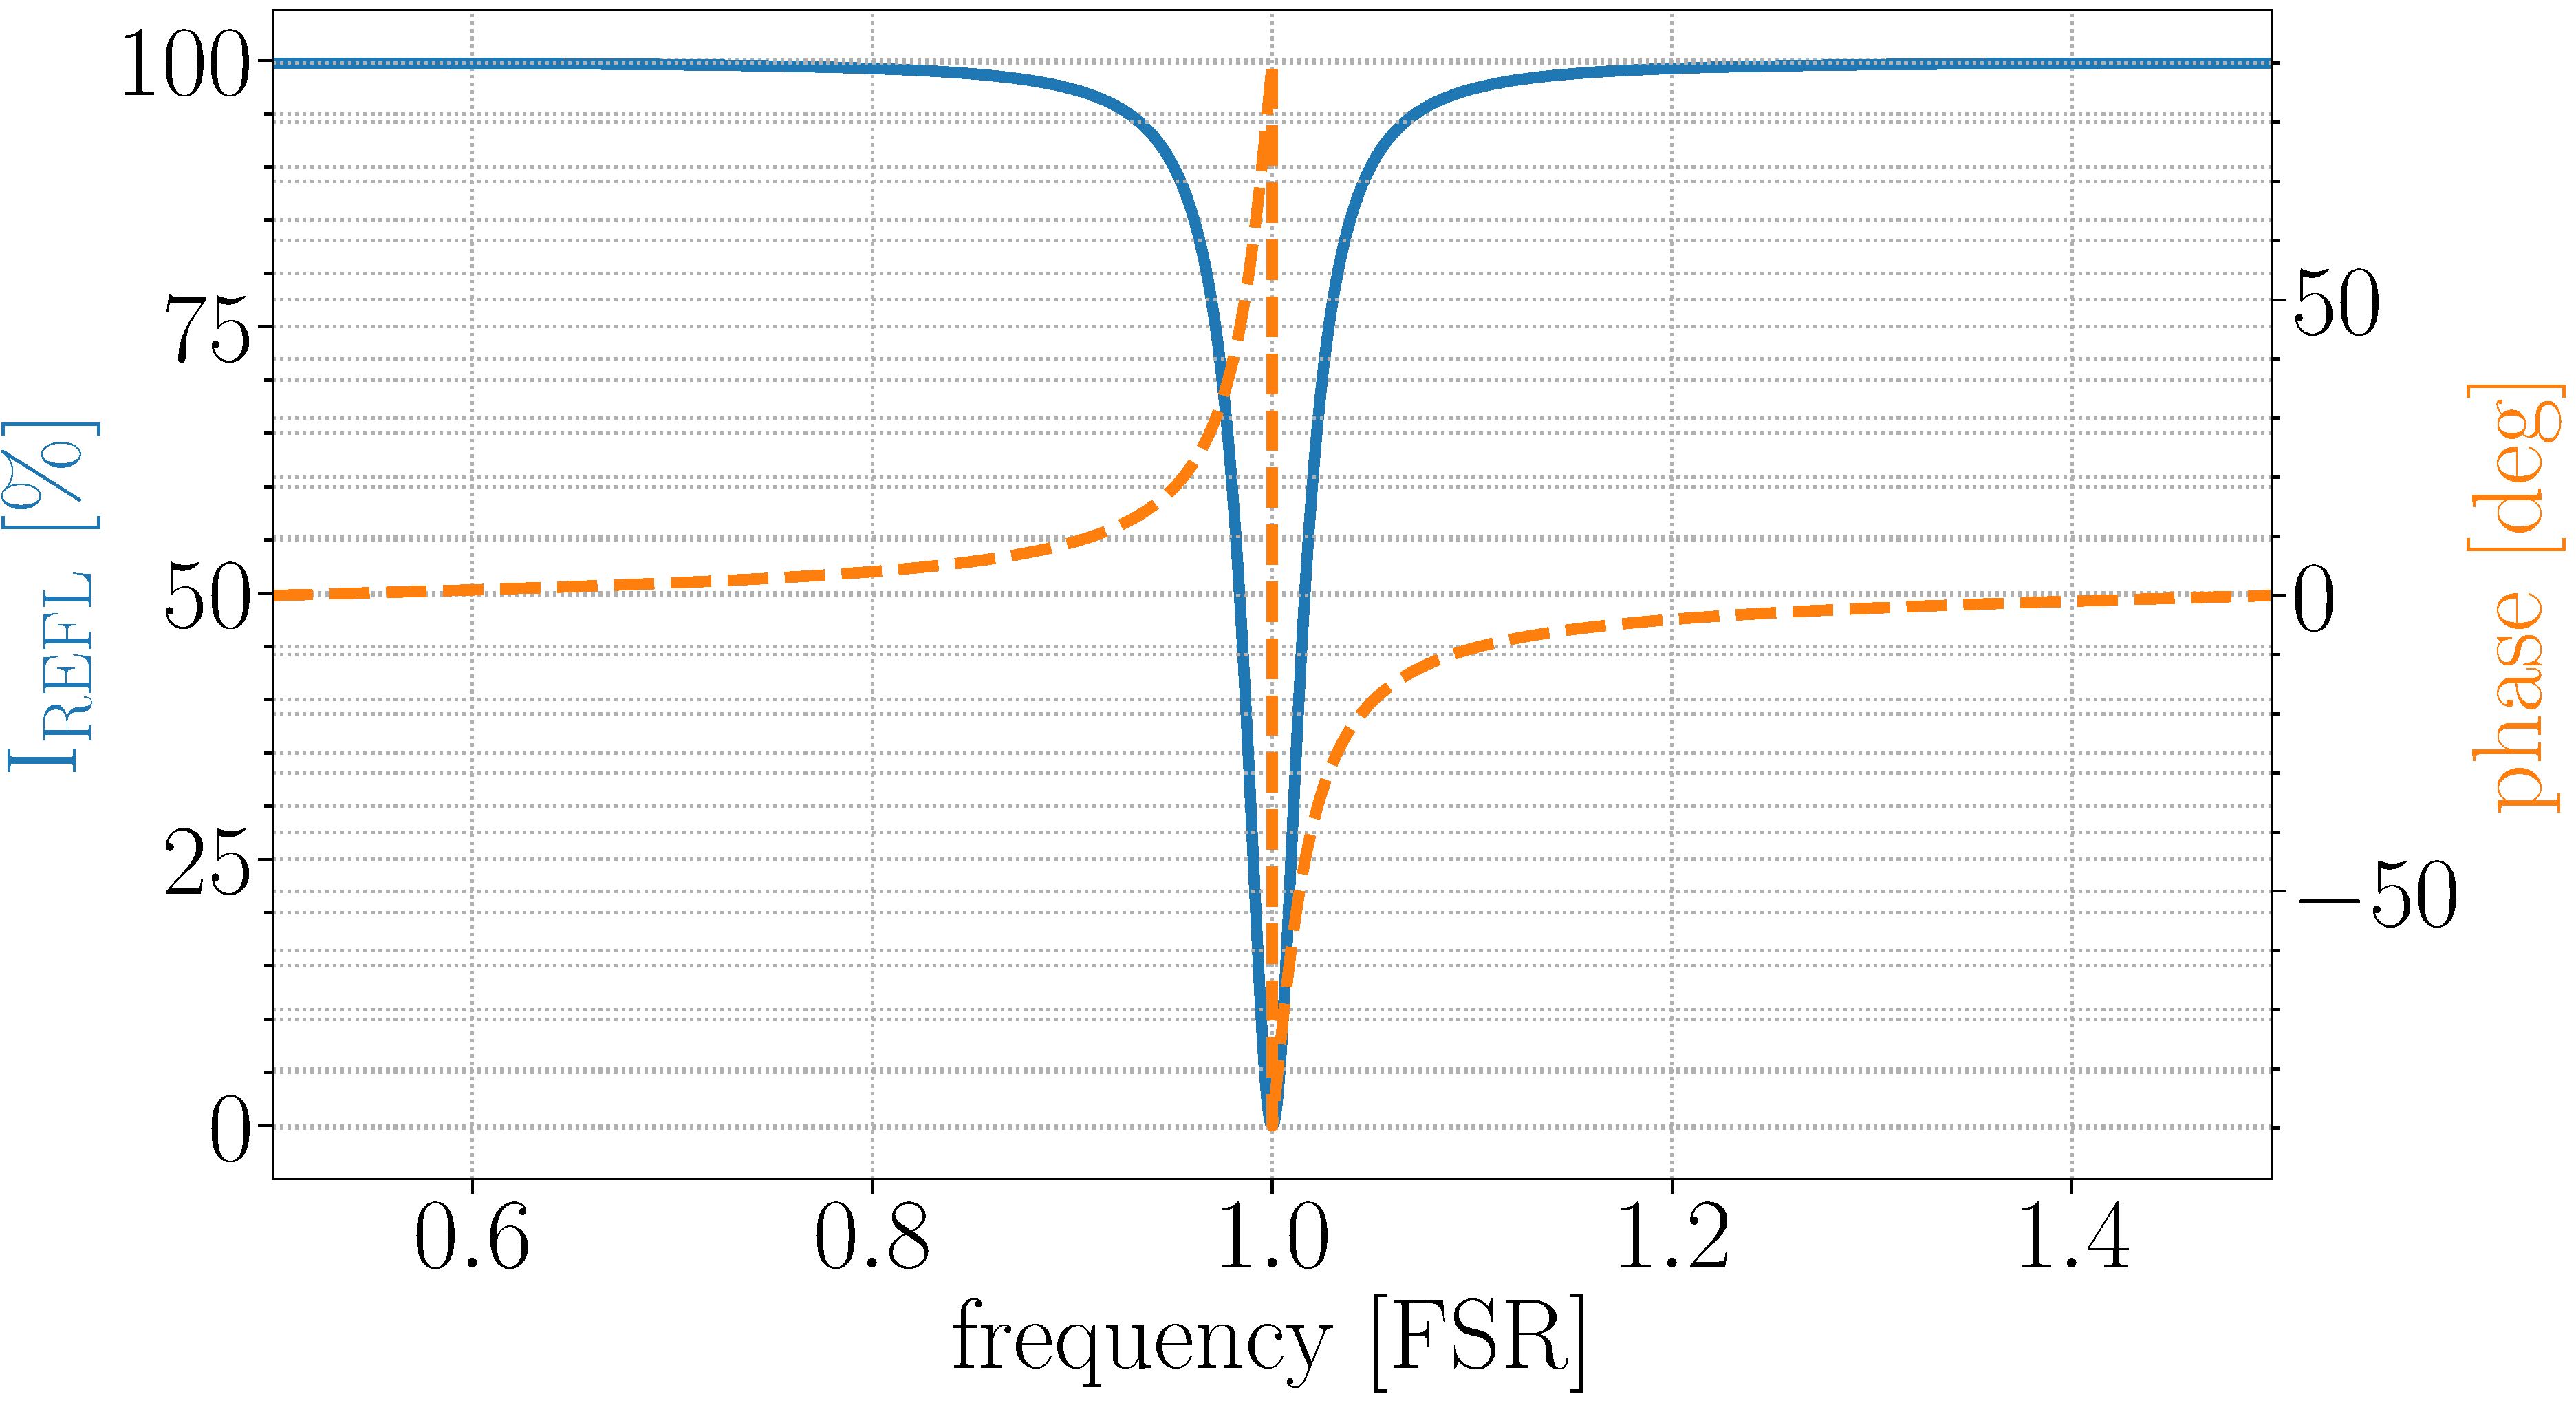
\includegraphics[width=\textwidth]{ALGAAS/REFL_cav_intensity.pdf}
\caption{Reflected cavity intensity (I$_\mathrm{REFL}$) around resonance. The resonance peak full width half maximum is set by mirror reflectivities and is succinctly quantified by the cavity \textbf{finesse} ($\mathscr{F} = \frac{\mathrm{FWHM}_\mathrm{res}}{f_\mathrm{FSR}} = \frac{\pi \sqrt{r_1 r_2}}{1-r_1 r_2}$).}
\label{fig:cav_length_response_DCpow}
\end{figure}

The ratio between circulating and cavity input power is set by the reflectivity paramters of the cavity mirrors, demonstrating the coorelation to how long a given phasefront can remain stored between said mirrors at resonance. This ``cavity storage time" ($\tau_s \appropto L r_1 r_2$) translates as a length elongation with the phasefront travel history encoded in the arrival time of its photons back at the beam splitter.

\begin{figure}[ht!]
  \begin{subcaptiongroup}{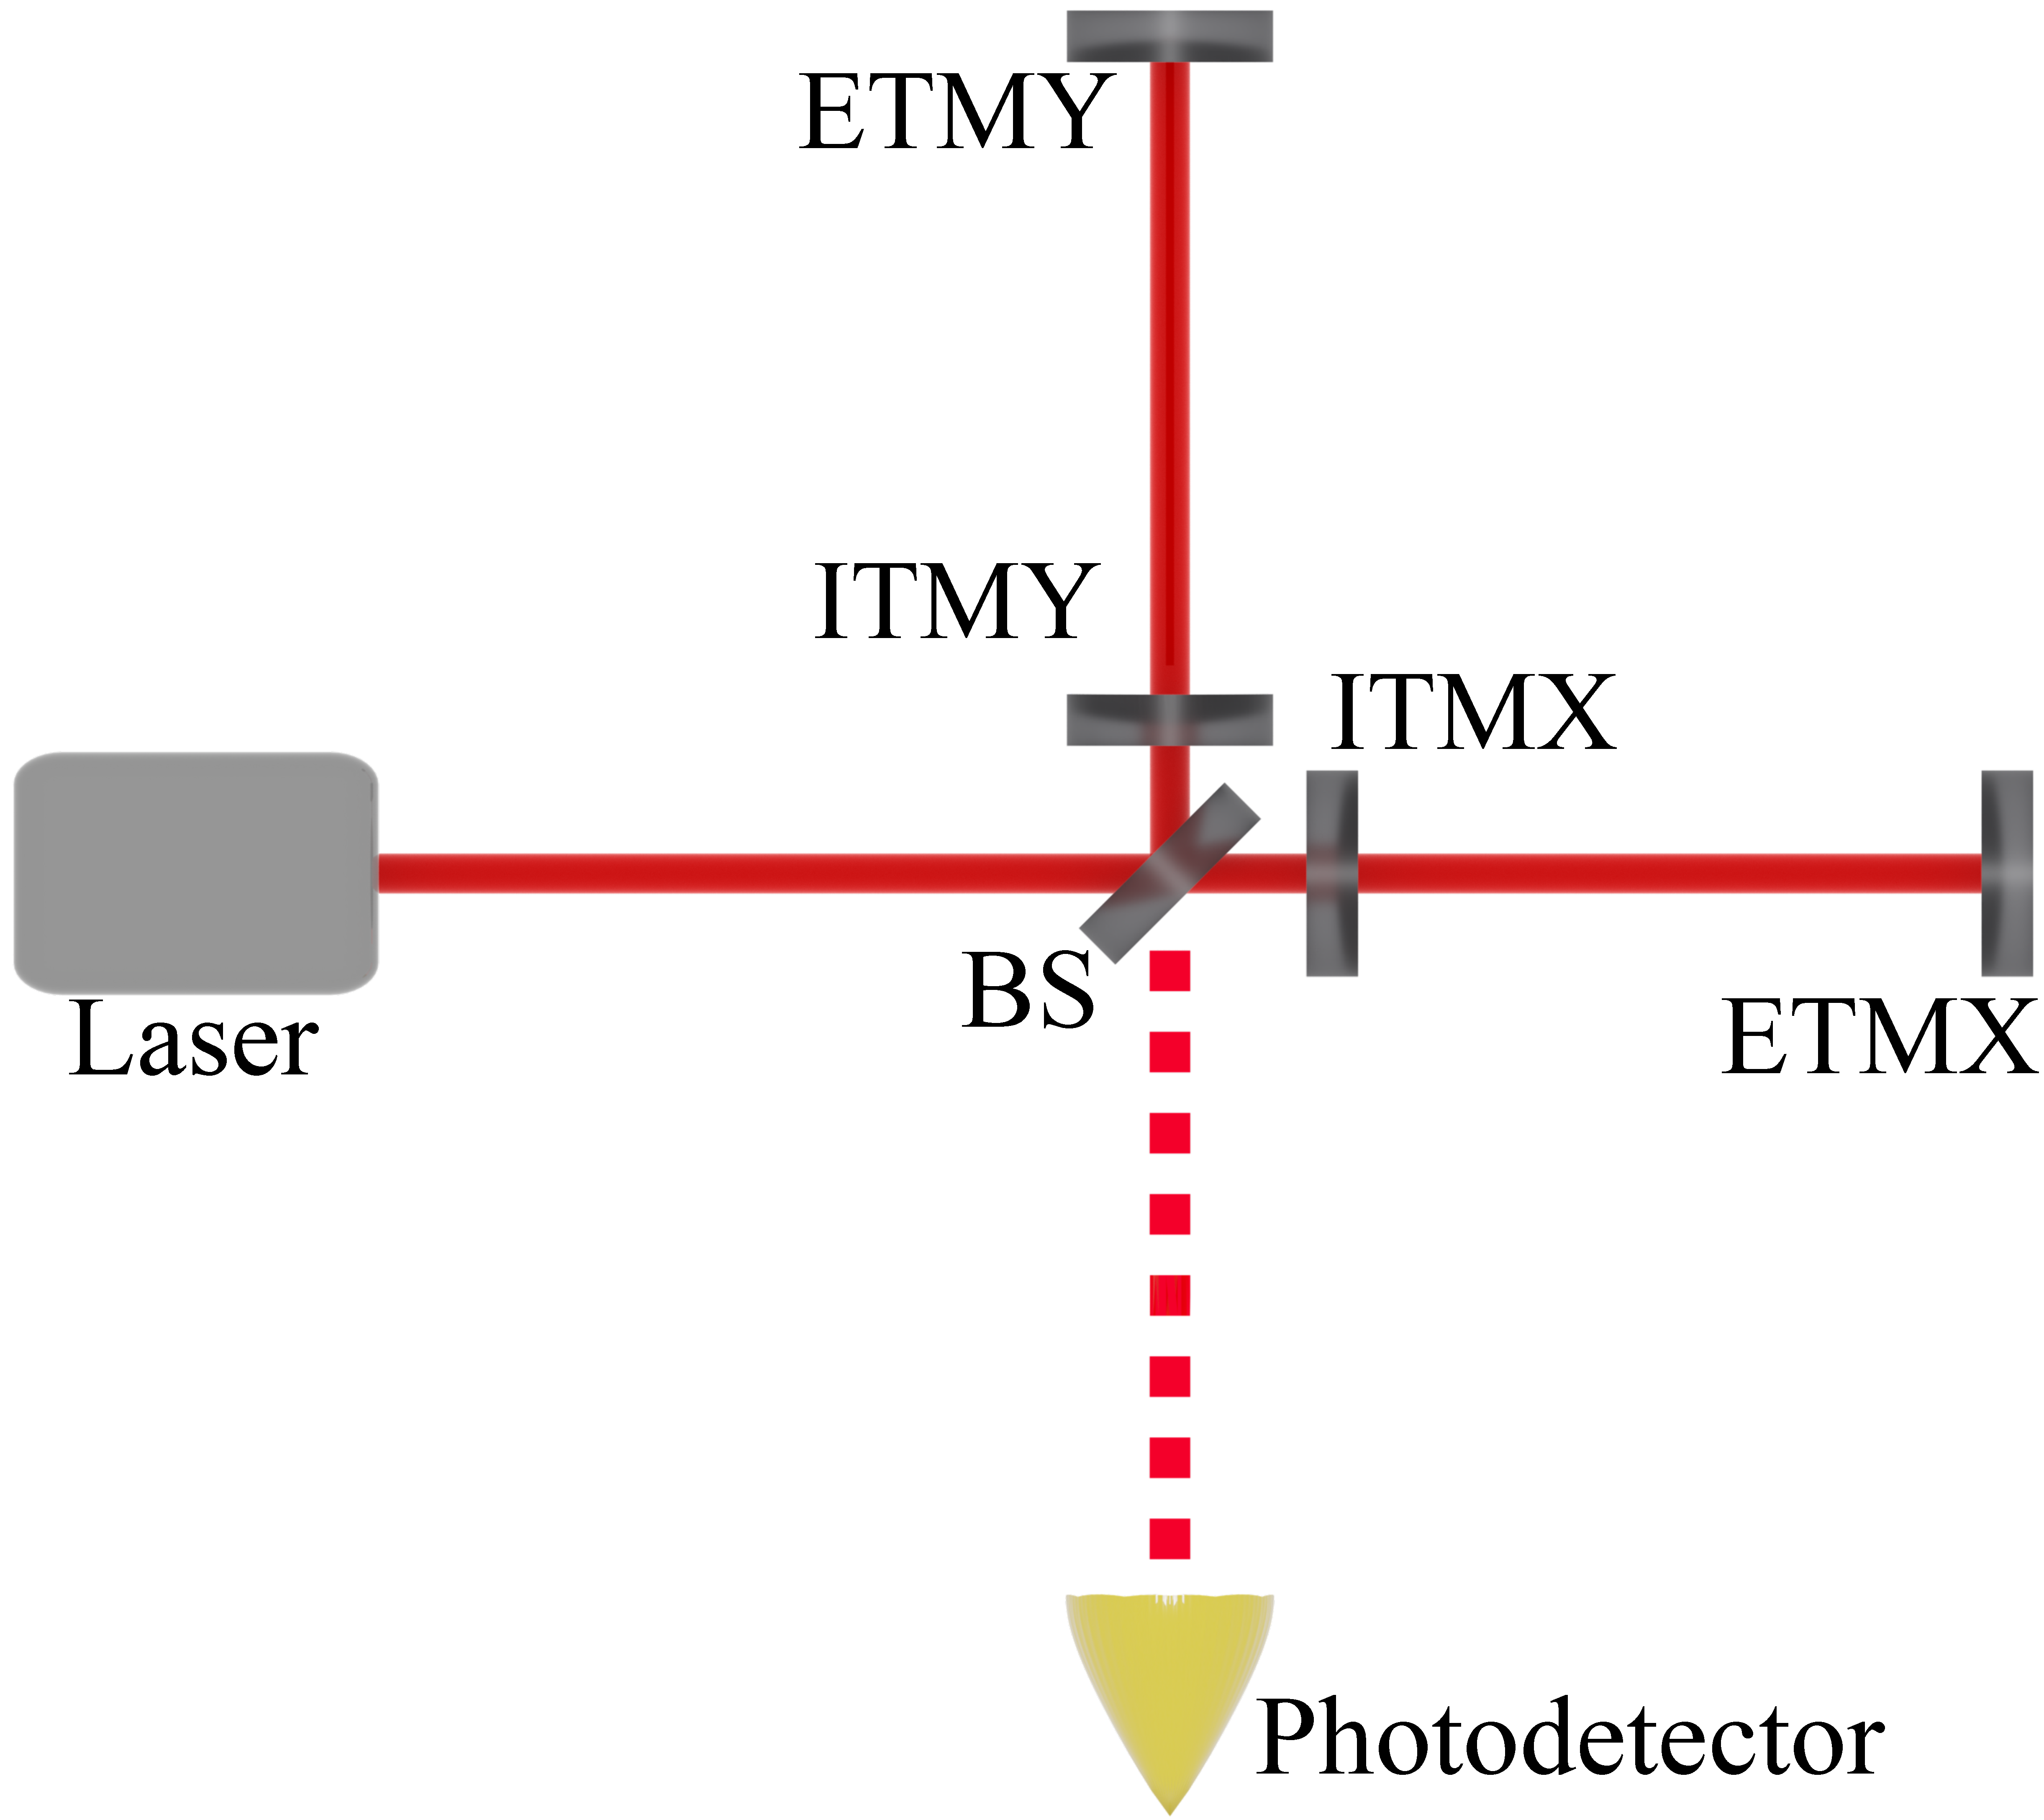
\includegraphics[width=.45\textwidth]{INTRO/fpmi_new.pdf}}
  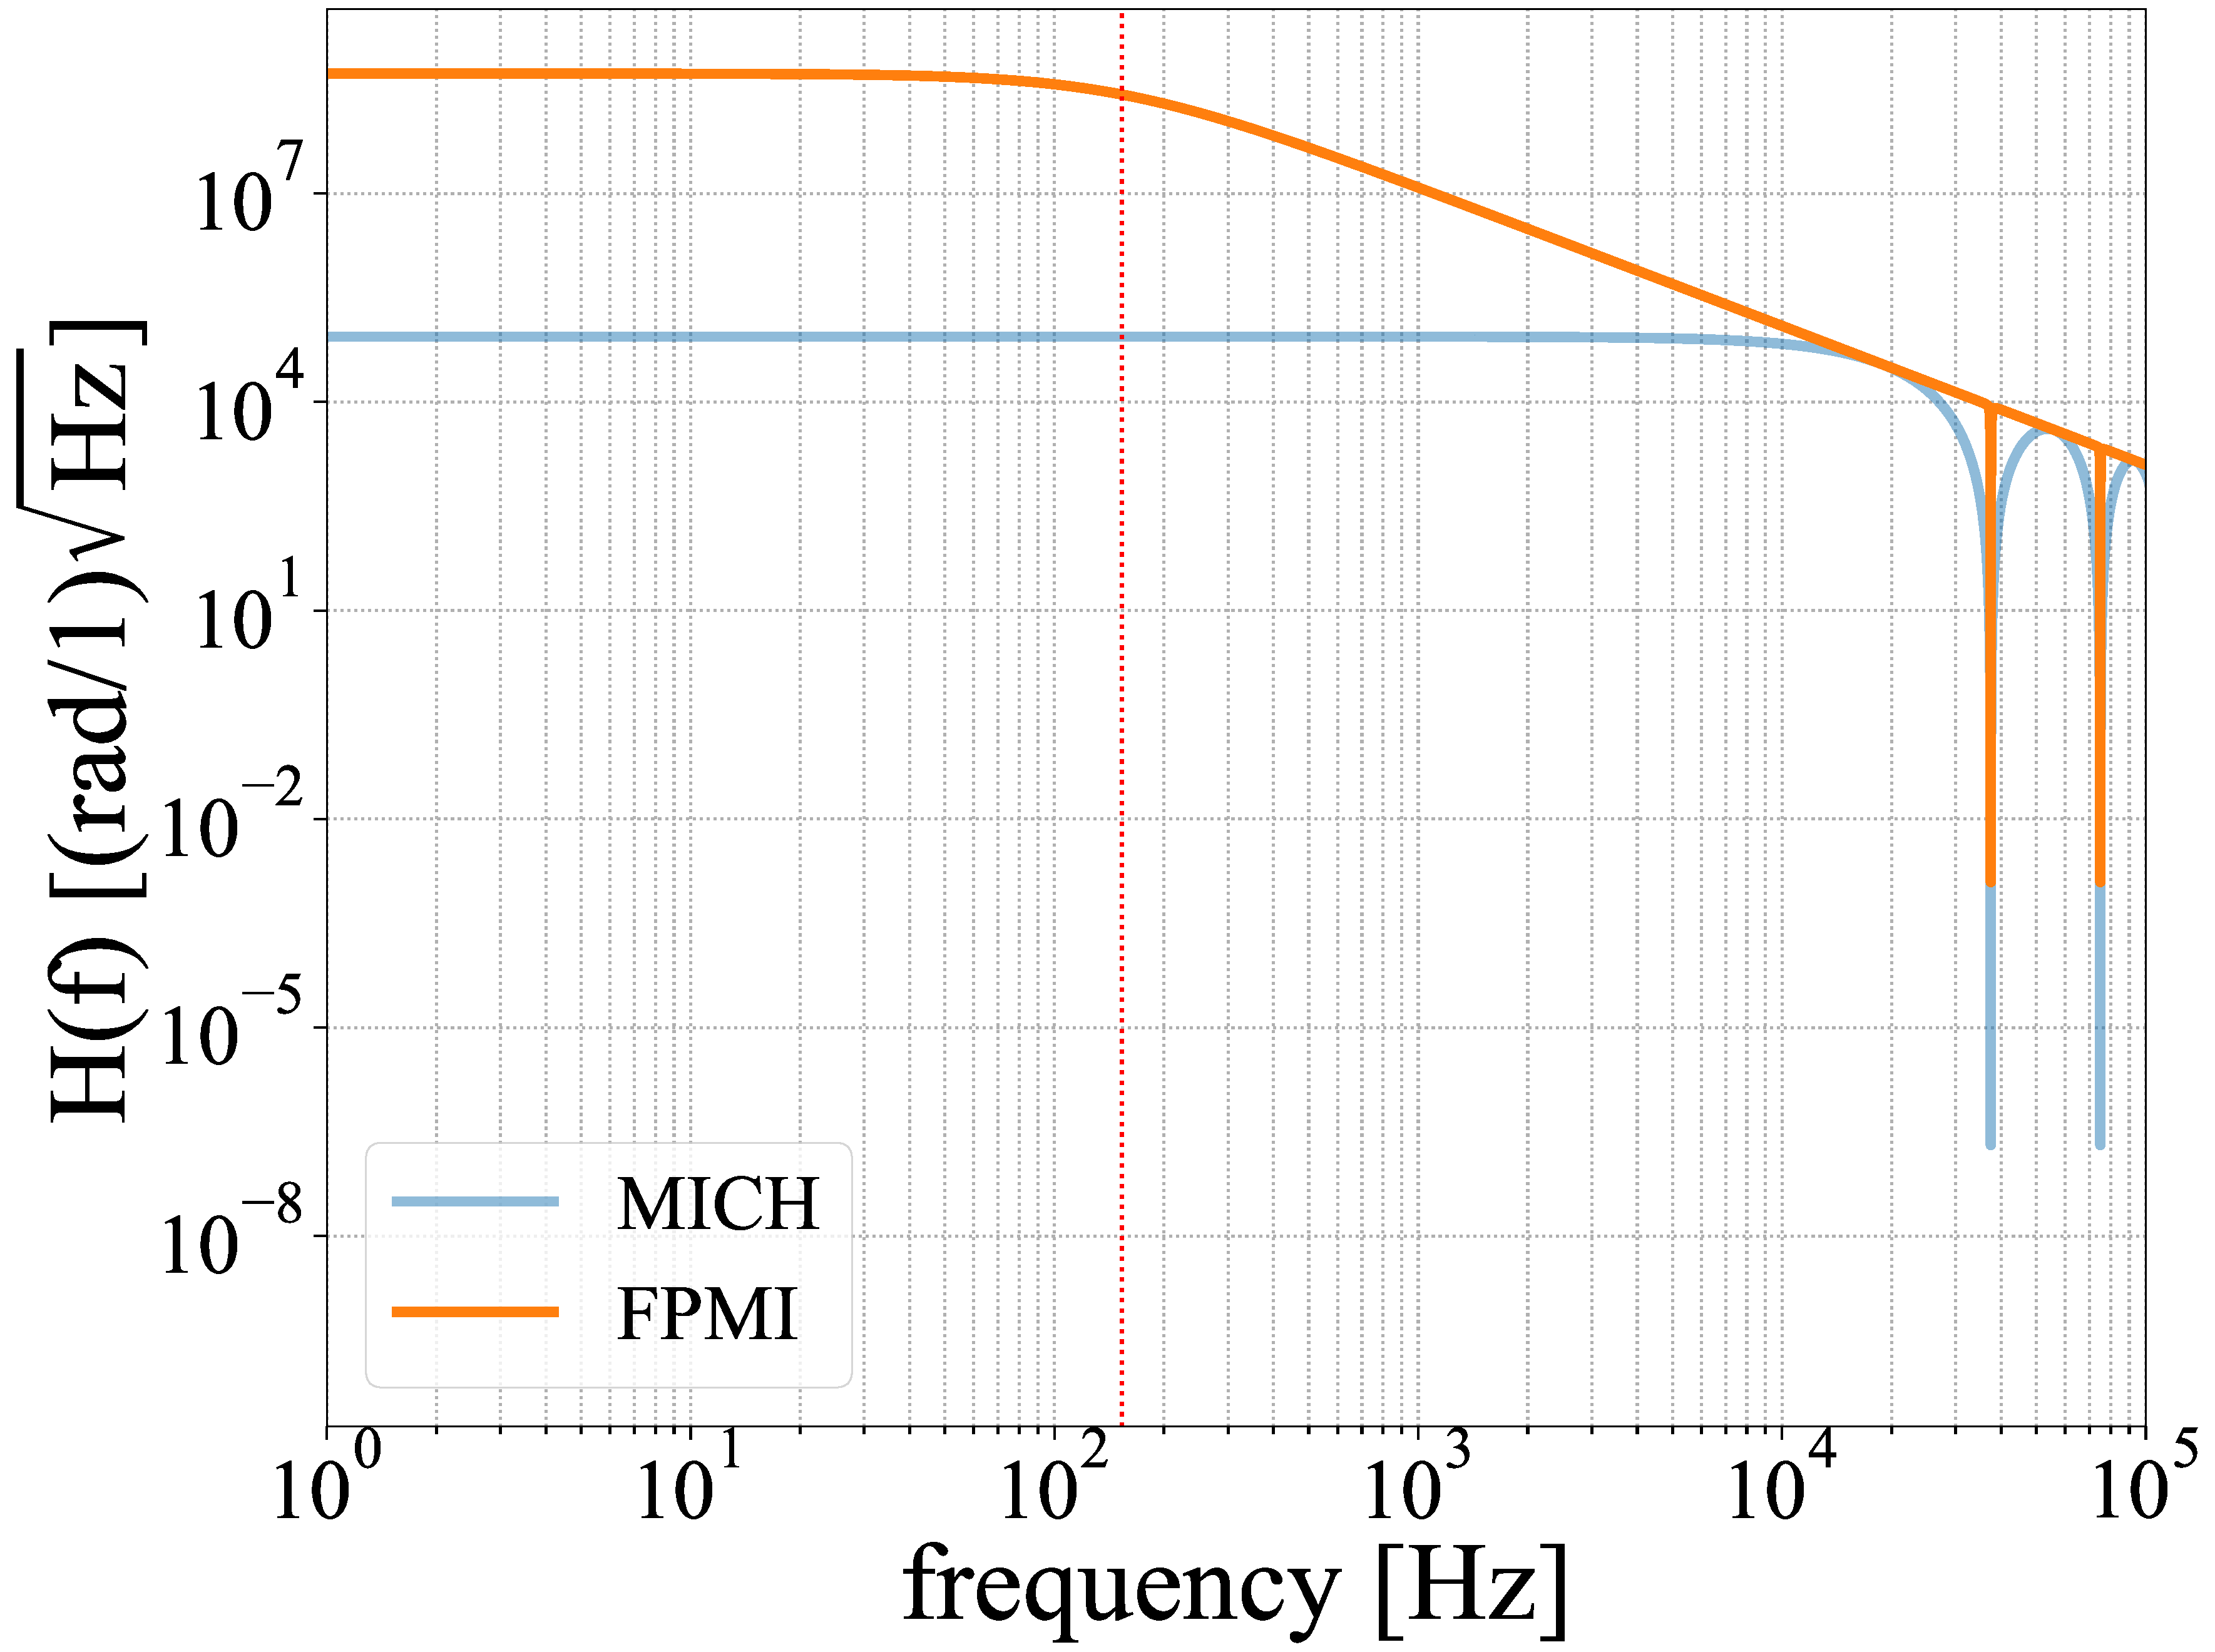
\includegraphics[width=.575\textwidth]{INTRO/fpmi_fr.pdf}
  \end{subcaptiongroup}
  \hfill
  \caption{[Left] The Fabry-P\'{e}rot Michelson optical schema and [Right] an associated optical gain.}
  \label{fig:fpmi}
\end{figure}

\paragraph{``Arm elongation''}

An intuitive analogue of the Fabry-P\'{e}rot's arm elongation capabilities is better illustrated when comparing against a computed Delay Line storage time (with $\mathscr{N}$ number of bounces and length L)~\cite{saulson:2017}:

\begin{equation}
    \tau^\mathrm{DL}_s = \frac{2 \mathscr{N} L}{c}
\end{equation}

\begin{equation}
    \tau^\mathrm{FP}_s = \frac{L}{c} \frac{r_1r_2}{1-r_1r_2} = \frac{1}{4 \pi \mathscr{F}}
\end{equation}

Advanced LIGO, with its 4km length and approximate finesse of 208 coorelates to a storage time of $382\mu s$, whereas the simple Michelson has an arm storage time of $26 \mu s$. The cooresponding optical gain increase is noted in \autoref{fig:fpmi}. 

\begin{equation}
	\mathrm{H_{FPMI}} = \frac{t_1 ^2 r_2}{(t_1^2 + r_1^2)r_2 - r_1} \frac{\mathrm{H_{MICH}}}{1 - r_1 r_2 e^{-2i \omega L / c}}
\end{equation}

The noted gain improvements made by adding two mirrors to the optical schema are substantial, though in practice the benefits are contingent upon: 1) maintaining fixed mirror positions within a fraction of the wavelength of the light used and 2) reducing detector bandwidth. But with tools like the Pound-Drever-Hall (PDH) technique and signal recycling to mitigate these respective burdens, it becomes clear that it is a small price to pay ~\cite{black:pdh}.

\paragraph{Gaussian and Higher Order Modes (Mode Matching pt.2)}\label{subsubsubsubsec:mm2}

There are some additional caveats before exploiting any potential enhancement from the Fabry-P\'erot when imposing a gaussian beam. First is that of beam divergence, which can quickly limit the stored power between two flat finite sized mirrors (see \autoref{sec:cavstab}). Though, as addressed for the simple Michelson, curving end mirrors focuses the Gaussian beam power and can also increase resonance robustness curving one or both cavity mirrors. 

Additionally mentioned is the importance of the overlap between mirror radii of curvature to the beam phasefront. For resonators this becomes increasingly critical as the placement of mirrors with established curvatures (defining the cavity mode) need to be placed such that they preserve the TEM00 beam mode. Beam optics inform solutions for optimal mirror placement for a given incident beam and vice versa. The exercise sets the importance of matching the \textbf{gaussian beam mode} to the spherical mirror \textbf{FP resonator mode}, but less obvious are the implications if there is a perturbation from the set solution. Alongside the TEM00 fundamental mode, the paraxial equation \autoref{sec:paraxial} also produces families of solutions that exist for the two mirror cavity configuration, characterized by the Hermite-Gauss and Laguerre-Gauss bases:

\paragraph*{Hermite-Gauss modes}

\begin{figure}[H]
	\centering
	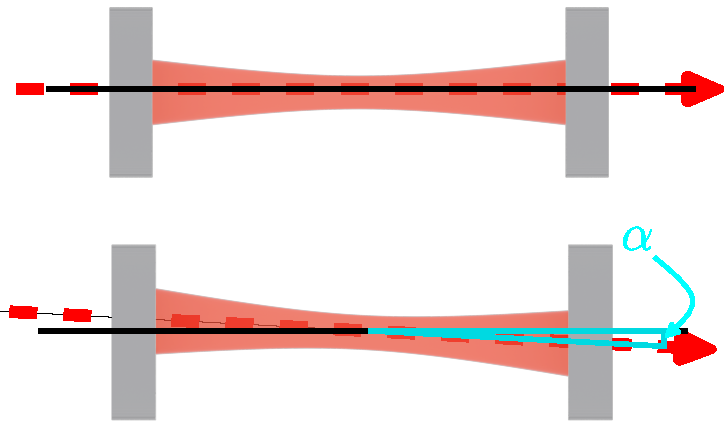
\includegraphics[width=.7\textwidth]{figs/INTRO/FP_misalignment.pdf}
	\caption{Figure depicting cavity-beam alignment (above) vs cavity-beam misalignment (below) with a angle $\alpha$ between the beam and cavity axes. }
	\label{fig:fp_misalignment}
\end{figure}

\begin{equation}\label{eq:HG_beam}
	\begin{split}
		TEM_\mathrm{n,m}(x,y,z) = & E_o \frac{\sqrt{[\lambda z_o] / \pi}}{W(z)}\mathbb{H}_\mathrm{n}\bigg(\frac{\sqrt{2}x}{W(z)}\bigg)\mathbb{H}_\mathrm{m}\bigg(\frac{\sqrt{2}x}{W(z)}\bigg)\\
					& \times \mathrm{exp}\bigg(\frac{-(x^2+y^2)}{W^2(z)}\bigg) \mathrm{exp}\bigg(-ikz - ik\frac{x^2 + y^2}{2R(z)} + i (1+\mathrm{n}+\mathrm{m})\zeta(z)\bigg)
	\end{split}
\end{equation}


As intensity, power and mode overlap are common computations, the gaussian integrals might be more quickly expressed and computed with the more conveniant bra-ket notation:

$$TEM_{n,m}(x,y,z) \rightarrow | U_\mathrm{n,m}(x,y,z)\rangle$$

\paragraph*{Laguerre-Gauss modes}
\begin{figure}[H]
\begin{subcaptiongroup}
	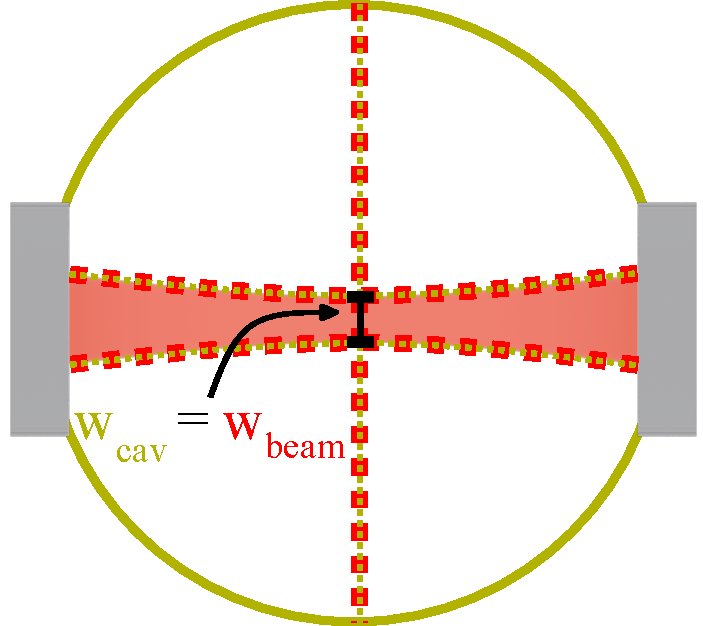
\includegraphics[width=.48\textwidth]{INTRO/FP_modematching.pdf}
	\hspace{3.5mm}
	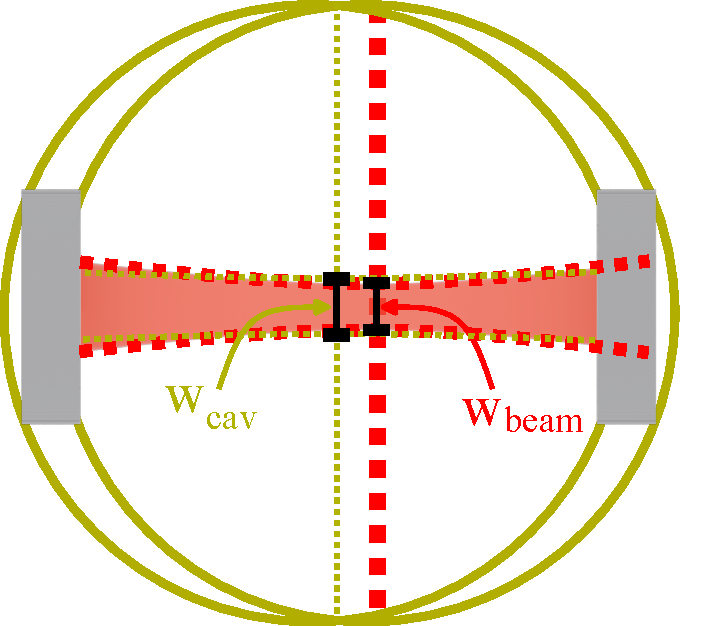
\includegraphics[width=.48\textwidth]{INTRO/FP_modemismatch.pdf}
\end{subcaptiongroup}
\hfill
\caption{Figure depicting cavity-beam mode matching (left) vs. cavity-beam mode mismatch (right). In this particular case, the mode mismatch is a result of changing the macroscopic DC cavity length via a shift of the ETM position towards the ITM (assuming constant mirror ROC and input beam mode). Given that the mirror ROC alongside the beam wavelength remains the same, it is helpful to notice that for the new cavity configuration, arriving at the same mirror ROC within the shorter length requires a larger characteristic beam waist (shortening the rayleigh length)}
\label{fig:fp_modemismatch}
\end{figure}

\begin{equation}\label{eq:LG_beam}
	\begin{split}
	TEM_\mathrm{p,l}(r,\phi,z) = & E_o \frac{\sqrt{[\lambda z_o] / \pi}}{W(z)} \bigg(\frac{\rho}{W(z)}\bigg)^\mathrm{p}\mathbb{L}^{\mathrm{p}}_{\mathrm{l}}\bigg(\frac{\sqrt{2}x}{W(z)}\bigg)\\
				   &  \times \mathrm{exp}\bigg(-\frac{\rho^2}{W^2(z)}\bigg) \mathrm{exp}\bigg(-ikz - ik\frac{\rho^2}{2R(z))} - i\mathrm{p}\phi + i (1+\mathrm{p}+2\mathrm{l})\zeta(z)\bigg)
	\end{split}
\end{equation}

$$TEM_{p,l}(r,\phi,z) \rightarrow | U_\mathrm{p,l}(r,\phi,z)\rangle$$


\begin{figure}[h!]
  \begin{subcaptiongroup}
	  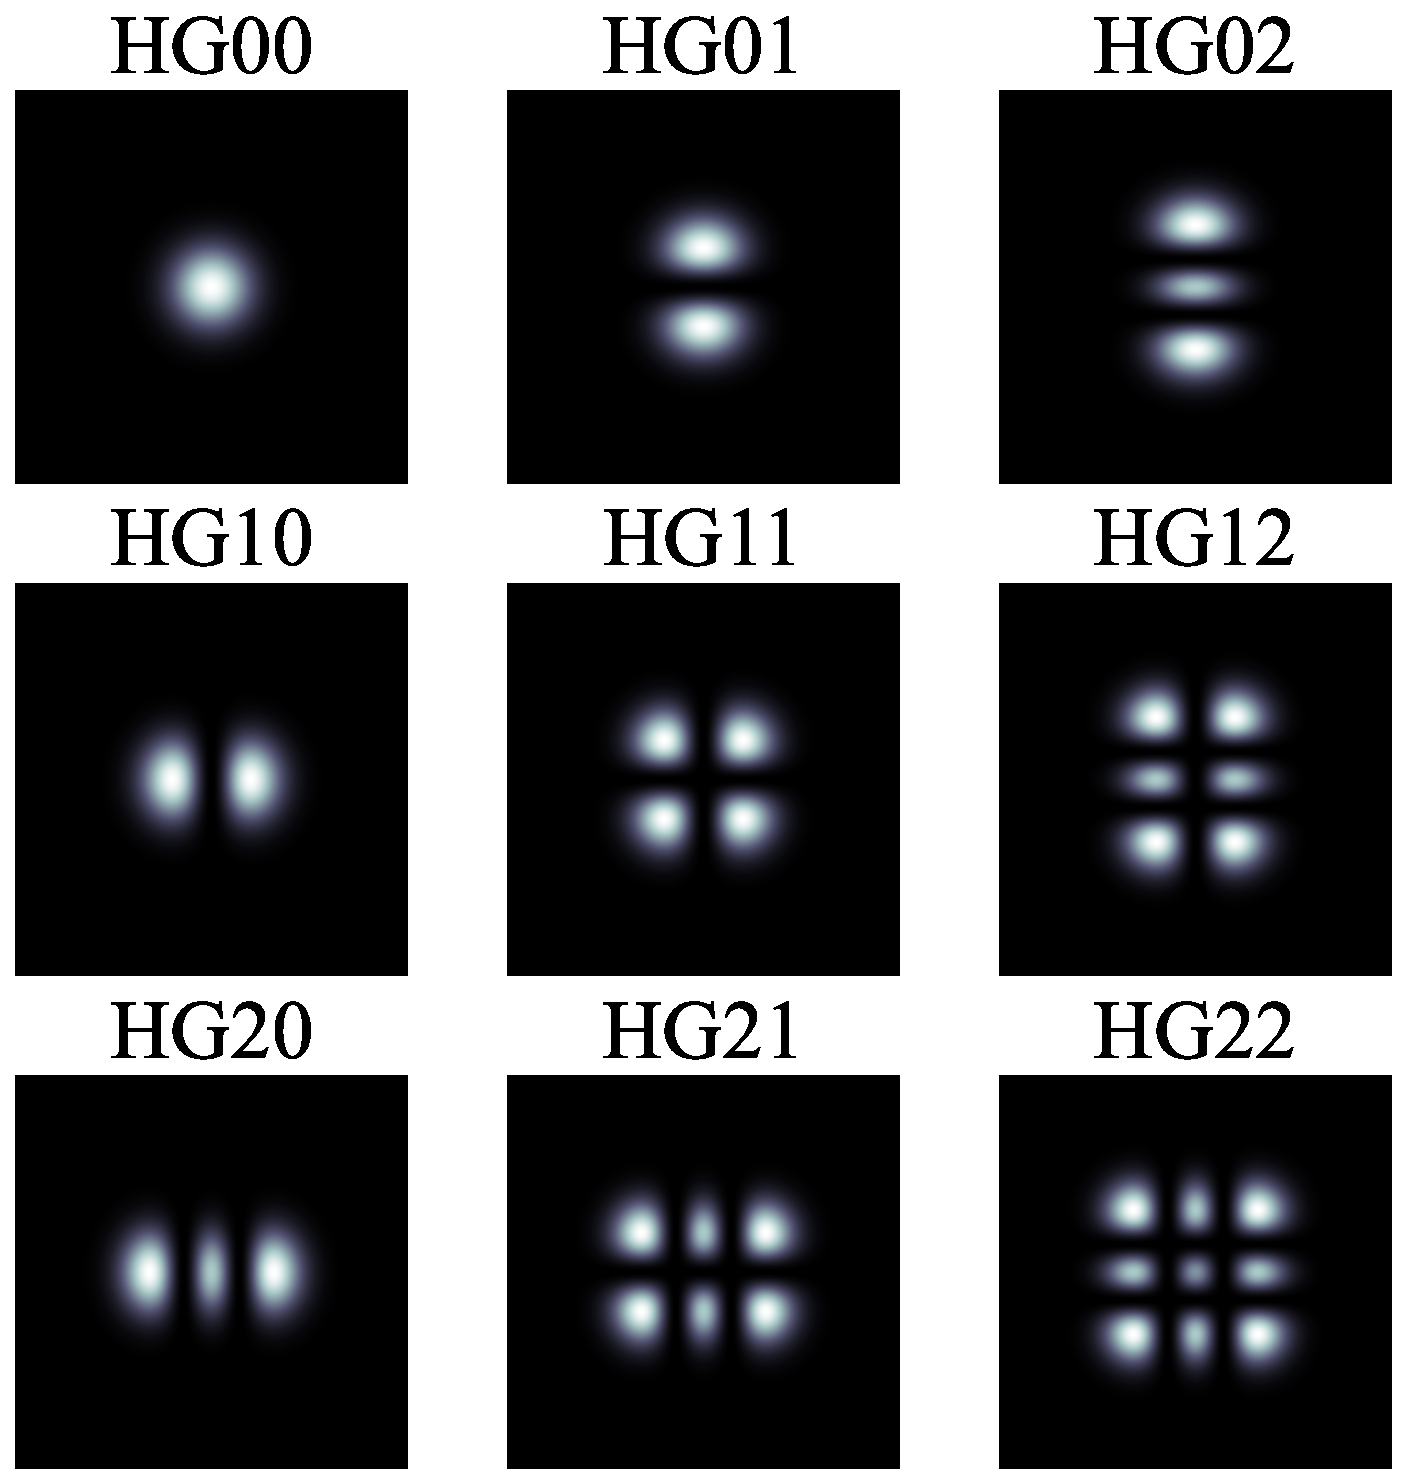
\includegraphics[width=.48\textwidth]{INTRO/HG00_HG22_modes.pdf}
	  \hspace{3.5mm}
	  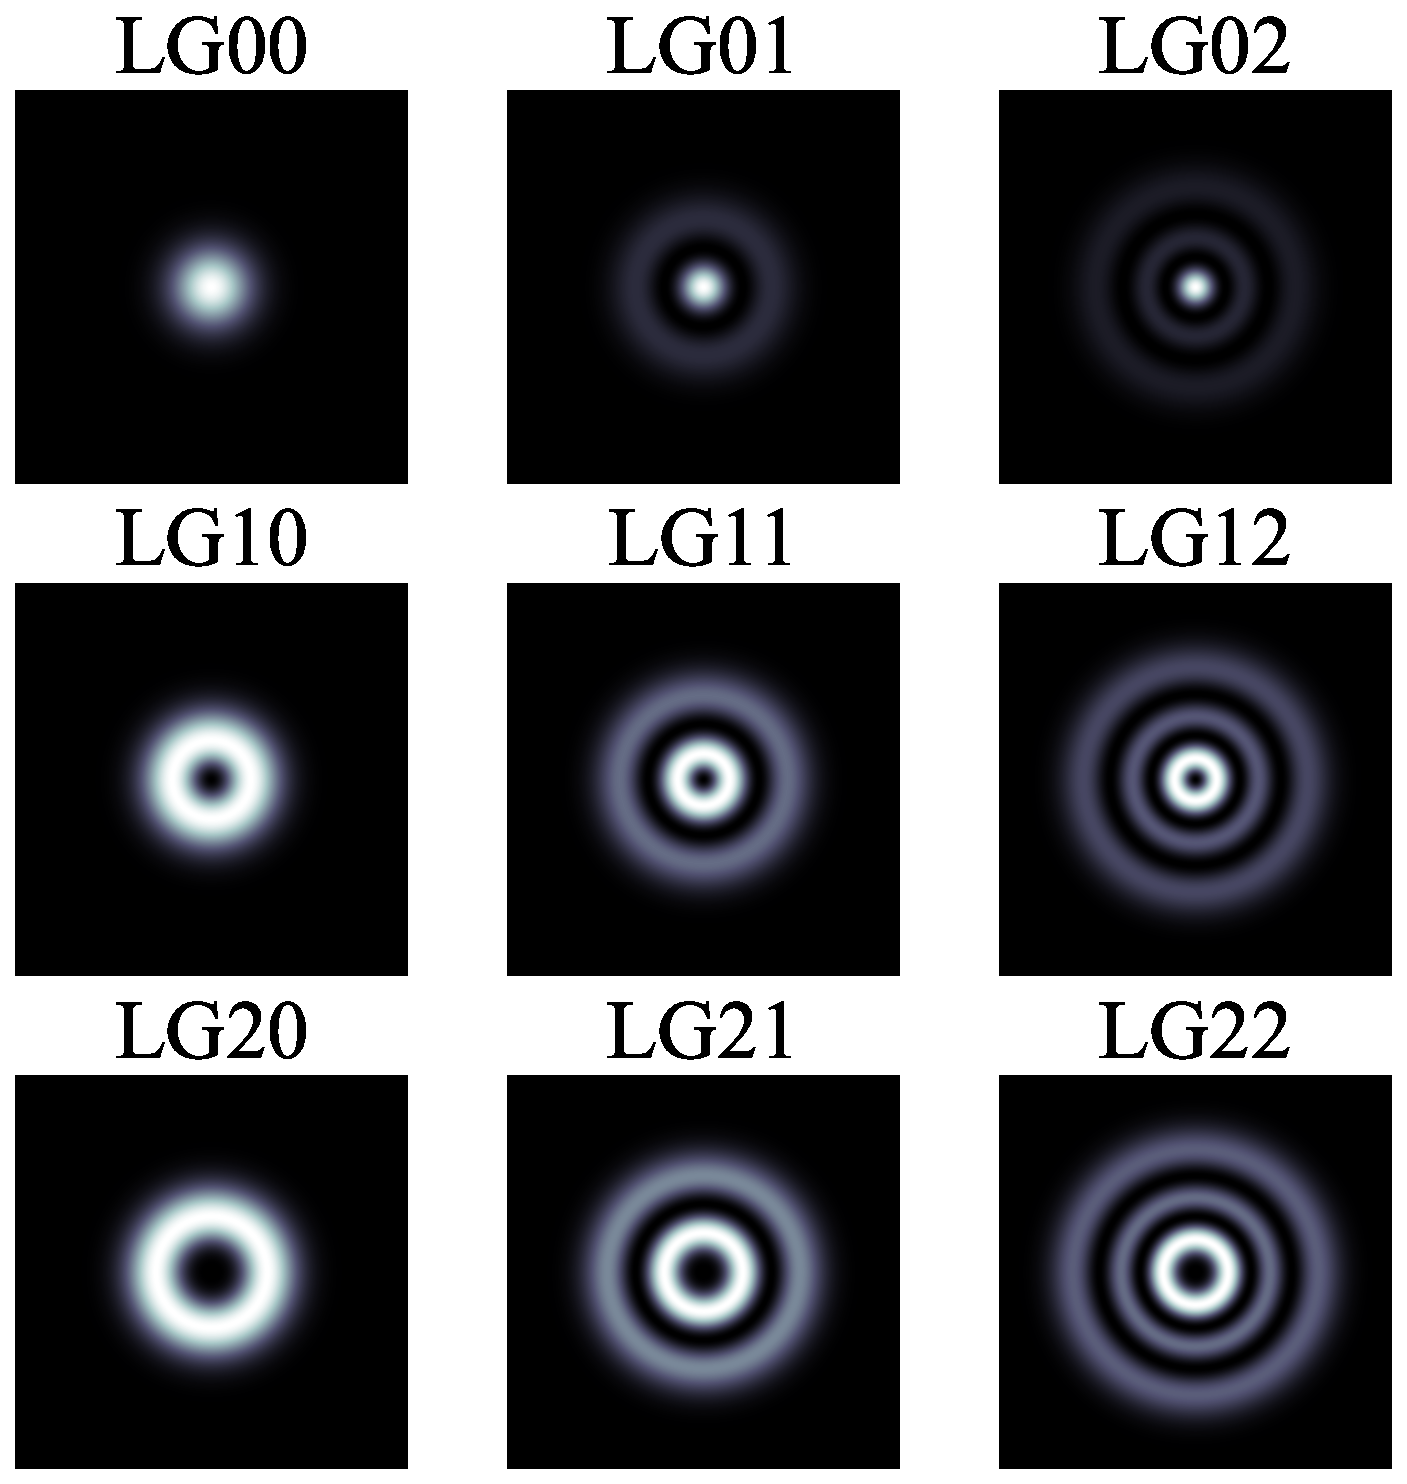
\includegraphics[width=.48\textwidth]{INTRO/LG00_LG22_modes.pdf}
  \end{subcaptiongroup}
  \hfill
  \caption{Various transverse mode intensity profiles, with Hermite-Gauss modes ($\mathrm{HG}_\mathrm{n,m}$, [n,m \hspace{.01pt} $\leq 2$]) to the left and Laguerre-Gauss modes ($\mathrm{LG}_\mathrm{l,m}$,  [l,m \hspace{.01pt} $\leq 2$]) to the right.}
  \label{fig:HGLG_modes}
\end{figure}

\newpage 
These HG and LG field solutions arise from added perturbations in the beam-cavity alignment and mode matching respectively. The presence of power in these modes when sweeping a mirror along the beam axis ($\Delta FSR$) indicate optical loss, while simultaneously providing useful feedback in reducing it through the construction and maintainence of a TEM00 beam-resonator coupling ~\cite{anderson:1984}. 

\subsection{Dual-Recycled Fabry-P\'erot Michelson (DRFPMI)}
Recycling mirrors are an extension of the FPMI that exploits otherwise wasted optical power by providing a means of enhancing the optical gain and bandwidth of the instrument. Strategic tuning of mirror coating parameters and positions at symmetric and anti-symmetric ports can incorporate power recycling and signal recycling respectively.

\begin{figure}[ht!]
\begin{center}
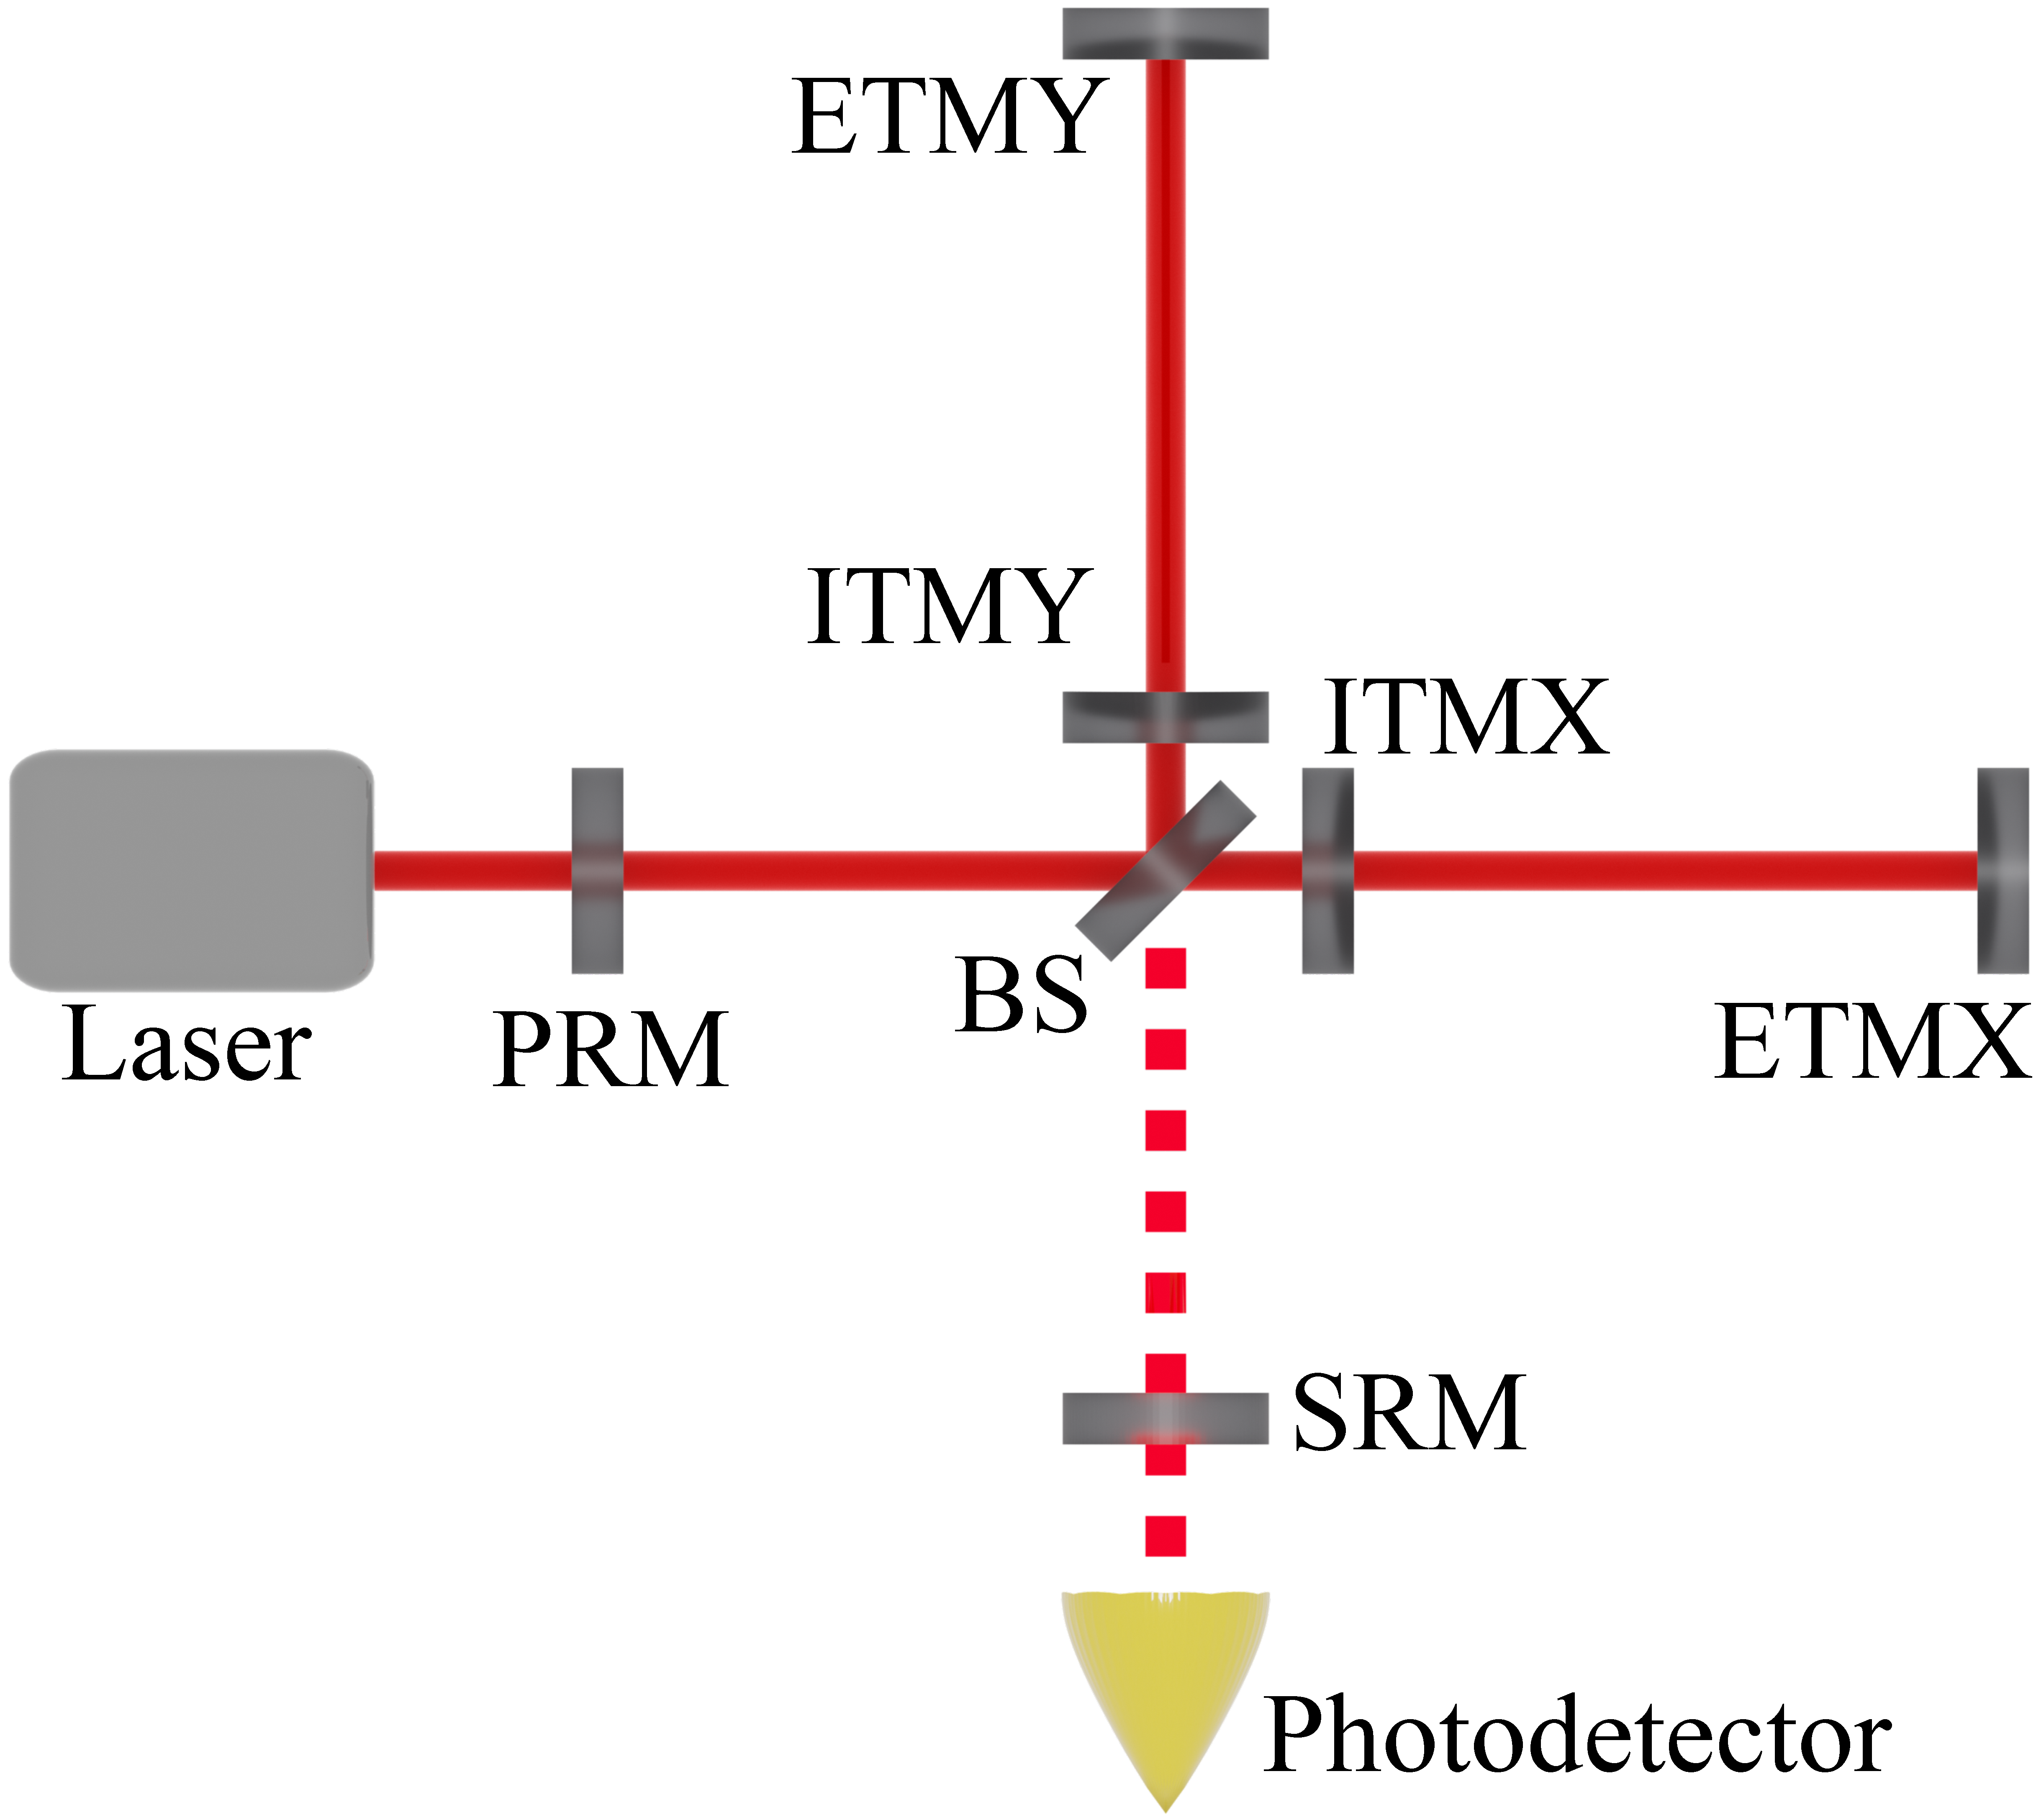
\includegraphics[width=\textwidth]{INTRO/drfpmi_new.pdf}
\end{center}
\caption{A simplified Dual-Recycled Fabry-P\'erot Michelson optical schema}
\label{fig:drfp_michelson}
\end{figure}

\subsubsection{Power Recycling}
When operating a FPMI at a dark fringe, a significant amount of power is reflected back to the symmetric port as mentioned in~\autoref{sec:FPC} leading to wasted optical power if simply dumped. Placing an additional highly reflective mirror at the symmetric port while maintaining resonance of the carrier to the arms, you can reintroduce (or ``recycle") power back to the arm cavities. A PDH loop is utilized for carrier resonance, while macroscopic mirror positioning of the PRM is informed by the choice of optical sideband frequency required when applying PDH. This recycling gain is also sensitive to cavity arm Finesse $\mathscr{F}$ and round trip loss $\mathscr{L}_\mathrm{RT}$: 

\begin{equation}\label{eq:PRG}
	\mathrm{G_{PR}} = \frac{(1-r_\mathrm{PRM}^2)}{1-r_\mathrm{PRM}[1- (\mathscr{F} \mathscr{L}_\mathrm{RT})/ \pi]}
\end{equation}

\noindent With maximum recycling gain: 

\begin{equation}
    \mathrm{G_{PR}}^{*} = \frac{\pi}{2 \mathscr{F} \mathscr{L}_\mathrm{RT}} \bigg[ \frac{1}{1- \frac{ \mathscr{F} \mathscr{L}_\mathrm{RT}}{ 2 \pi}} \bigg]
\end{equation}

\subsubsection{Signal Recycling}
As may be inferred, this technique requires a mirror installation at the anti-symmetric port, though with a more nuianced approach than that of power recycling. Placing a partially reflective mirror at the output port, it is understood that light leakage coming from the PRFPMI at the anti-symmetric port (caused by differential arm motion) is re-introduced to the arms, but the reflectivity of the new mirror cannot be set too high to prevent attenuating the PRFPMI output. And even then detector enhancement only comes after exacting a cost dependent on signal recycling cavity tuning. This cost resides between a trade off of detector bandwidth for increased detector gain or vice versa, with the operating point between the maxima of these two detector characteristics set as a function of the microscopic signal recycling cavity length (phase) tuning ~\cite{Vajente:2018_unpub}:

\begin{equation}
	\mathrm{H}_\mathrm{DRFPMI} = \mathrm{G}_\mathrm{PR} \mathrm{P}_\mathrm{in} L \Omega \bigg[ \frac{ t_\mathrm{ITM}^2 r_\mathrm{ETM}}{(t_\mathrm{ITM}^2 + r_\mathrm{ITM}^2)r_\mathrm{ETM} - r_\mathrm{ITM}}  t_\mathrm{SRC} \frac{e^{-i 2 \pi L f / c} \mathrm{sin}( 2 \pi f / c)}{ 2 \pi L f } \frac{\mathrm{sin}(\phi_0)}{1- r_\mathrm{SRC}r_\mathrm{ETM} e^{-i 4 \pi L f / c}} \bigg]
\end{equation}

\begin{align}
	t_\mathrm{SRC} & = \frac{t_\mathrm{SRM} t_\mathrm{ITM} e^{i\phi_\mathrm{SRC}}}{1-r_\mathrm{ITM} r_\mathrm{SRM} e^{i2\phi_\mathrm{SRC}}}, \\
	r_\mathrm{SRC} & = \frac{r_\mathrm{ITM} - r_\mathrm{SRM} e^{i2\phi_\mathrm{SRC}}}{1-r_\mathrm{ITM} r_\mathrm{SRM} e^{i2\phi_\mathrm{SRC}}} 
\end{align}

\begin{figure}[h!]
  \begin{subcaptiongroup}
	  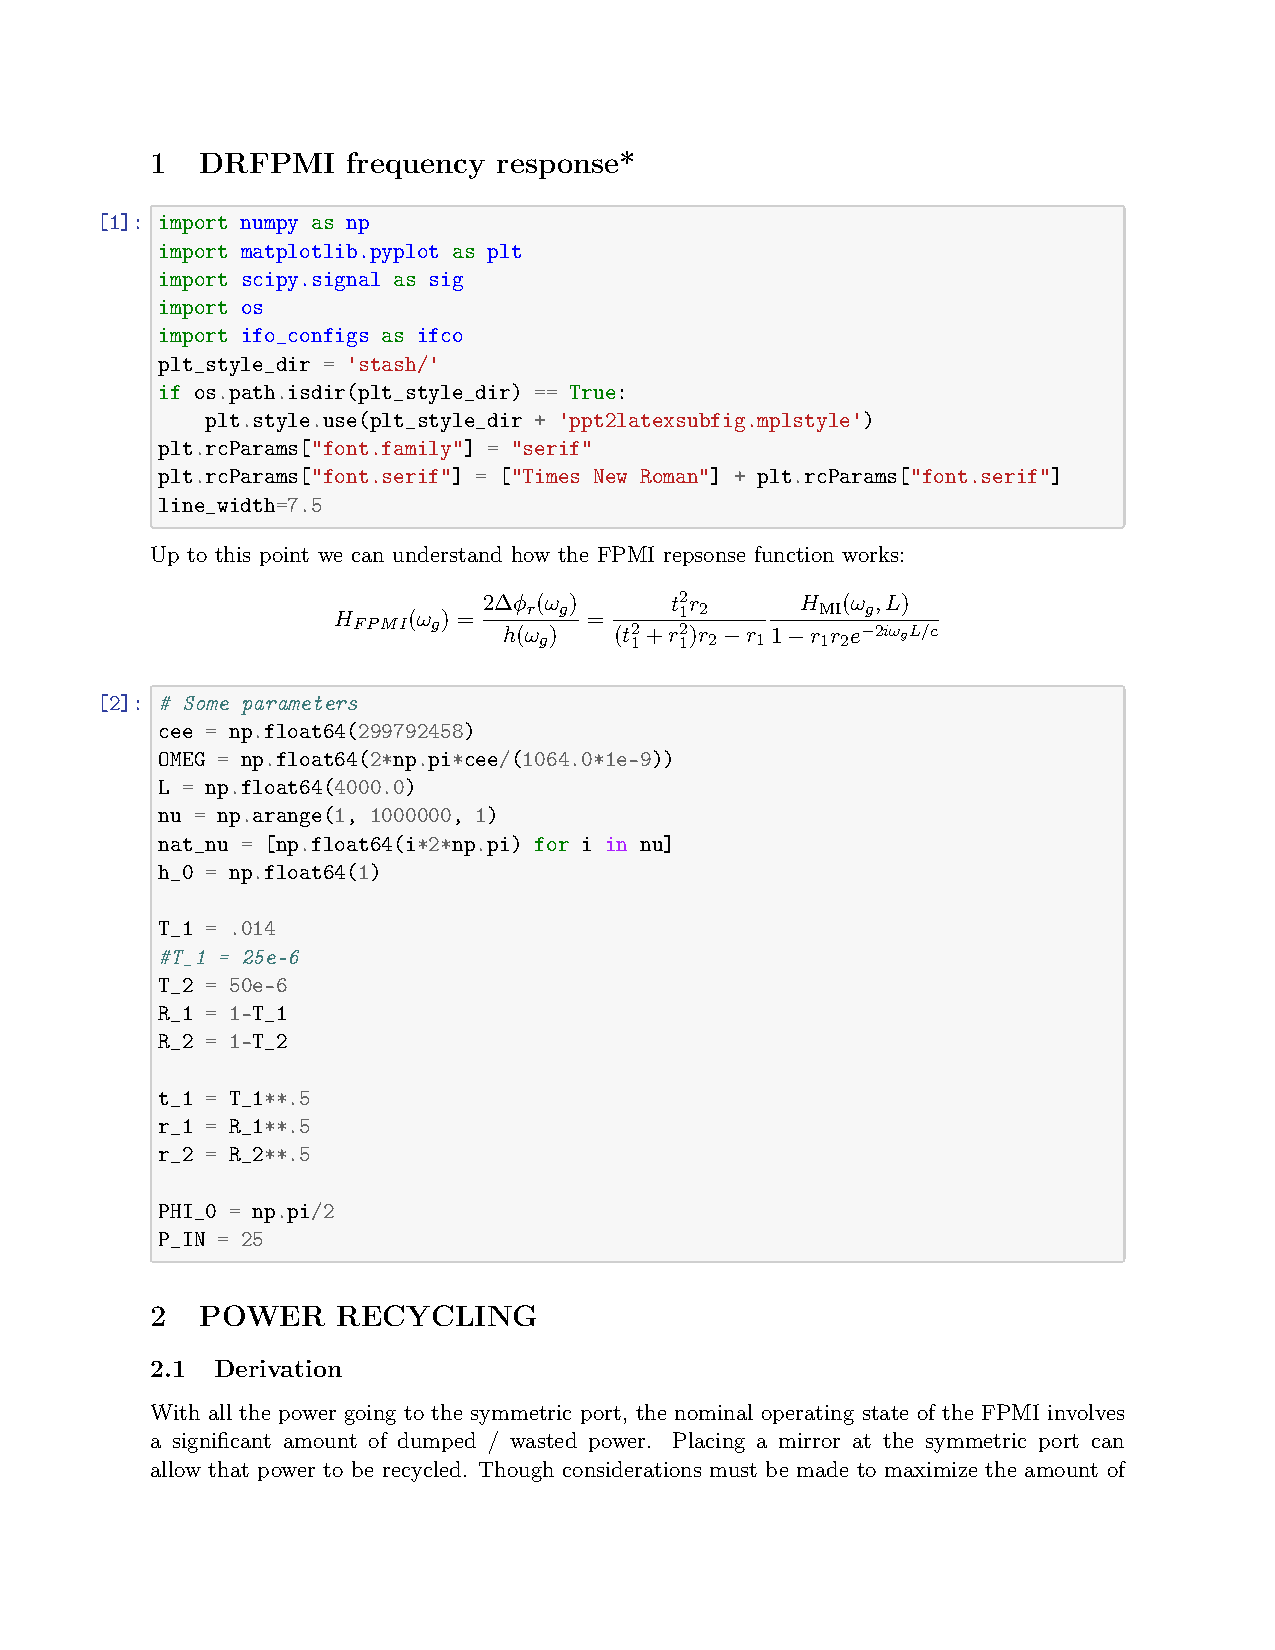
\includegraphics[width=.487\textwidth]{INTRO/drfpmi_fr.pdf}
 	  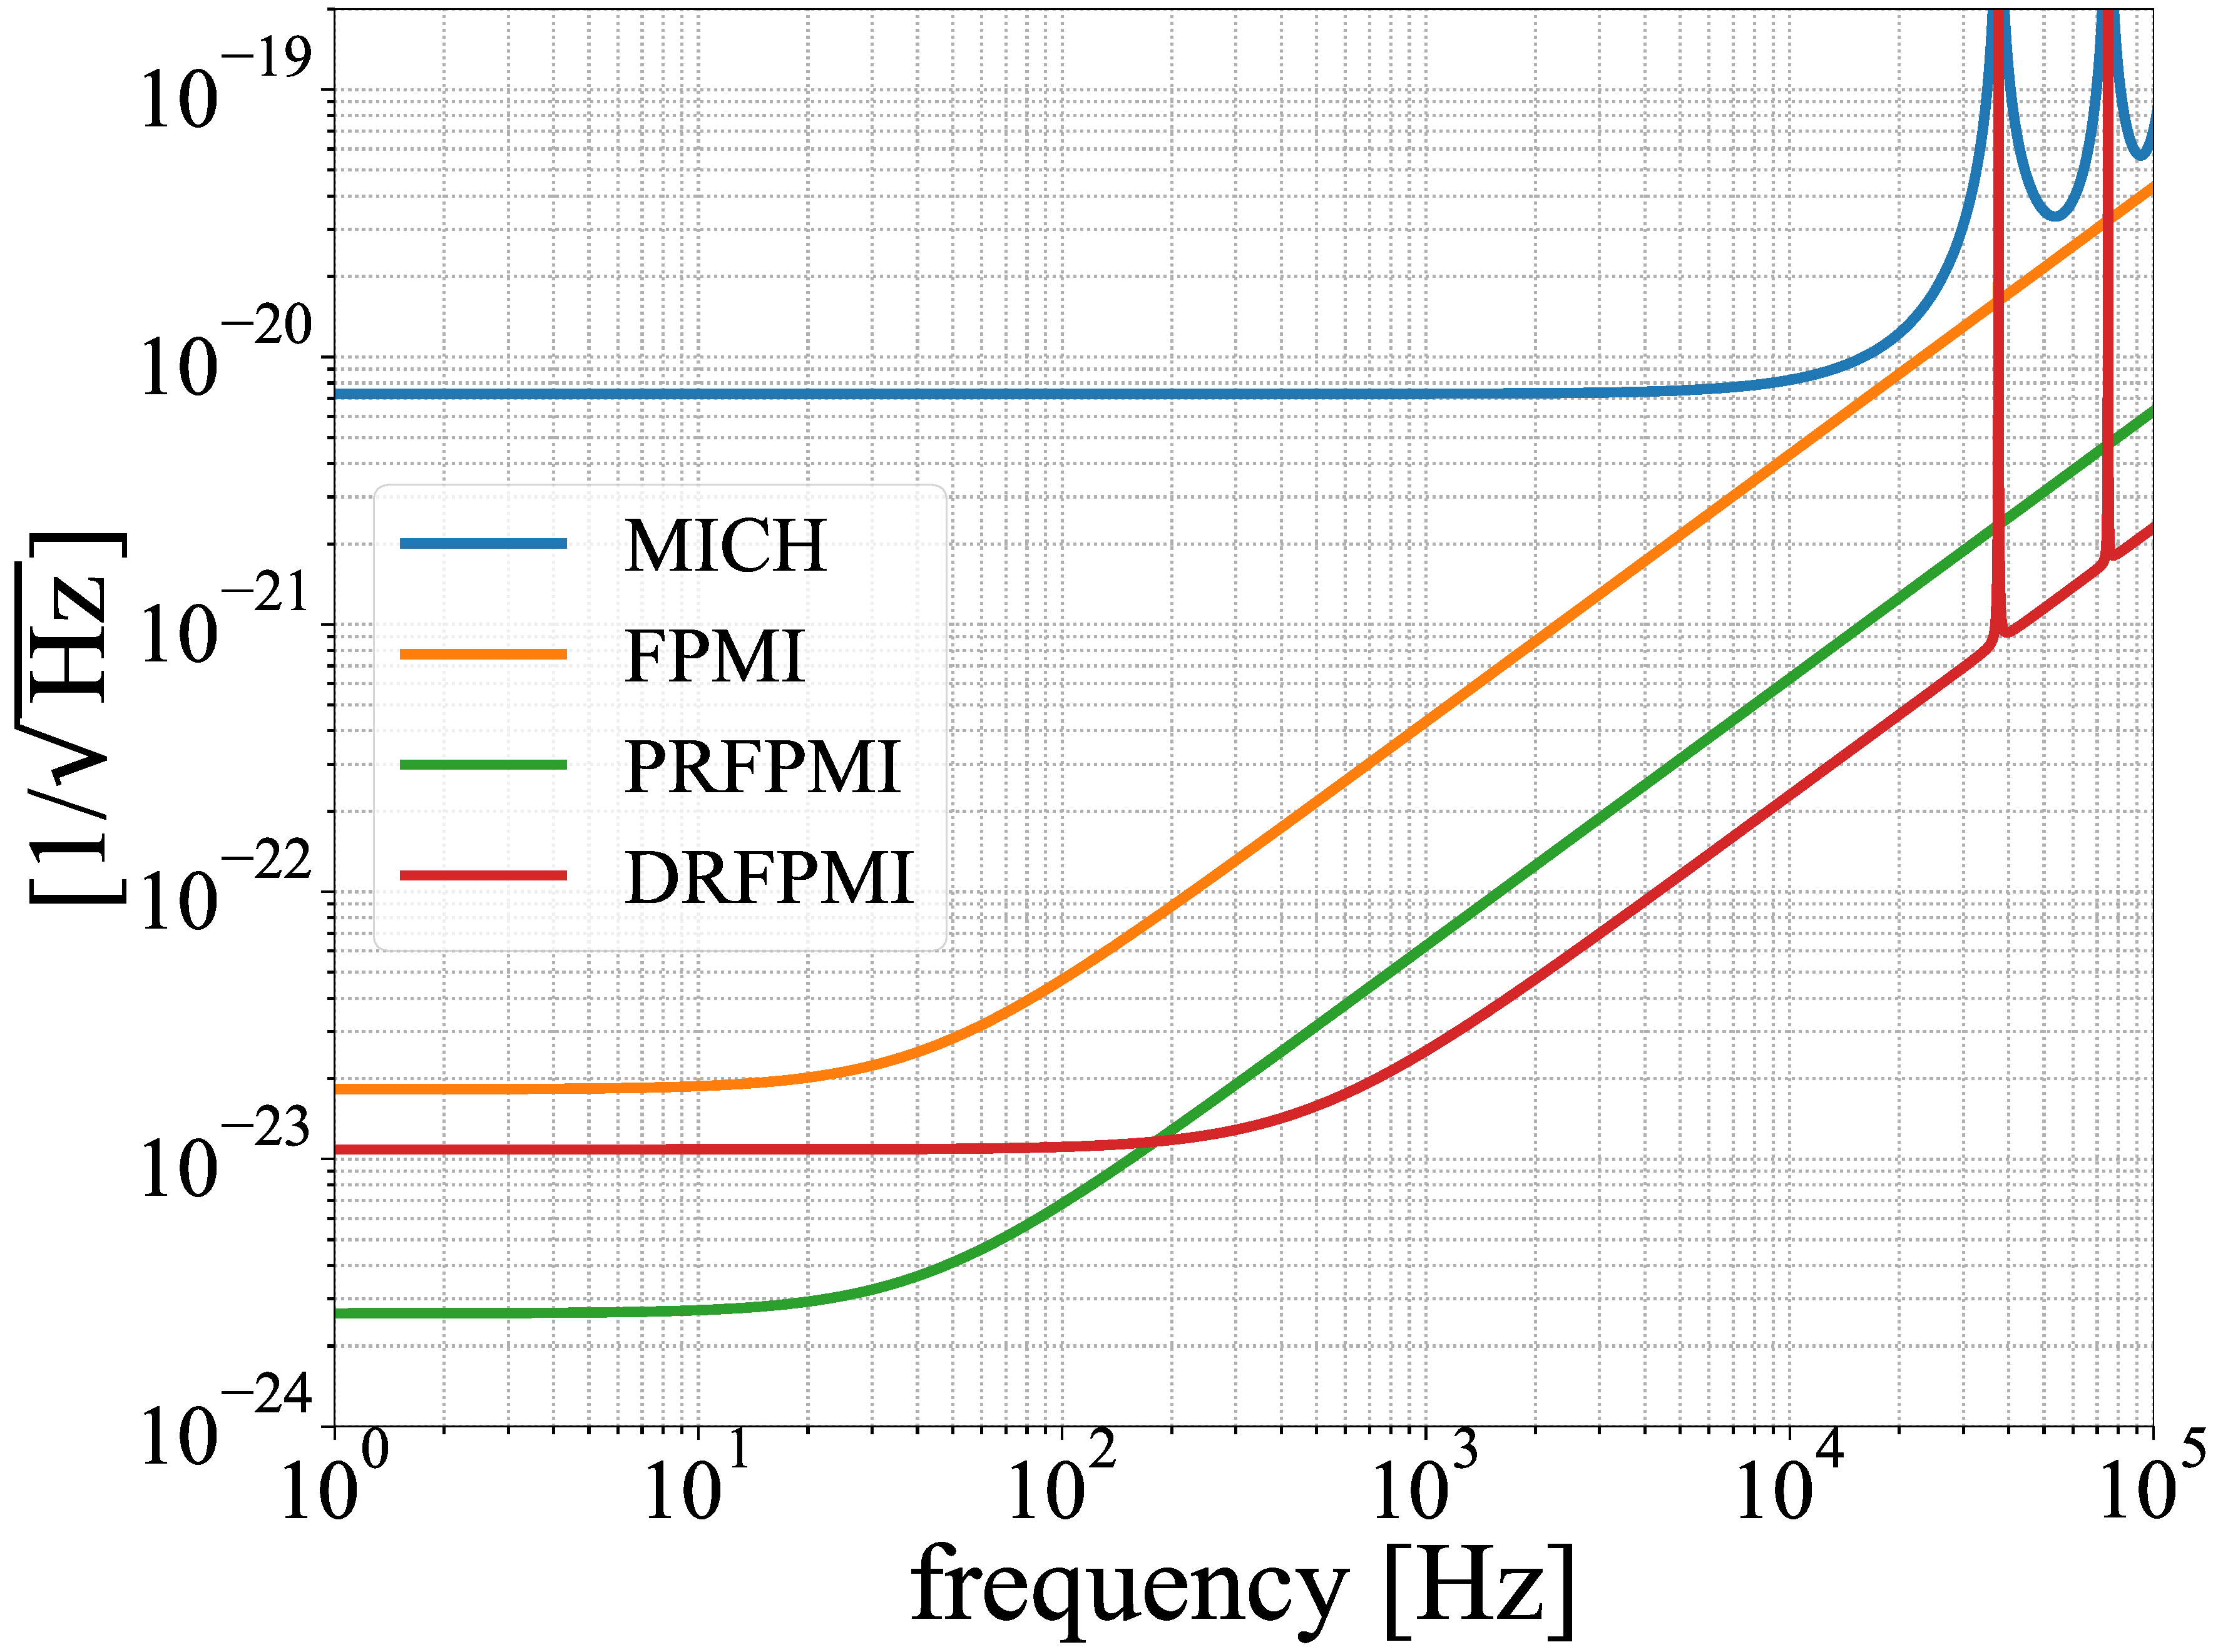
\includegraphics[width=.5\textwidth]{INTRO/strain_compare.pdf}
  \end{subcaptiongroup}
  \hfill
  \caption{[Left] Comparison of all optical gain functions [Right] Coorelated shot noise strain sensitivity. Code and more detailed derivations used to generate optical gain and sensitivity curves can be found in \autoref{appendix:ifo_configs_code}}
  \label{fig:drfpmi_gain_and_strain}
\end{figure}

\section{ALIGO}

\begin{figure}[H]
  \begin{center}
	  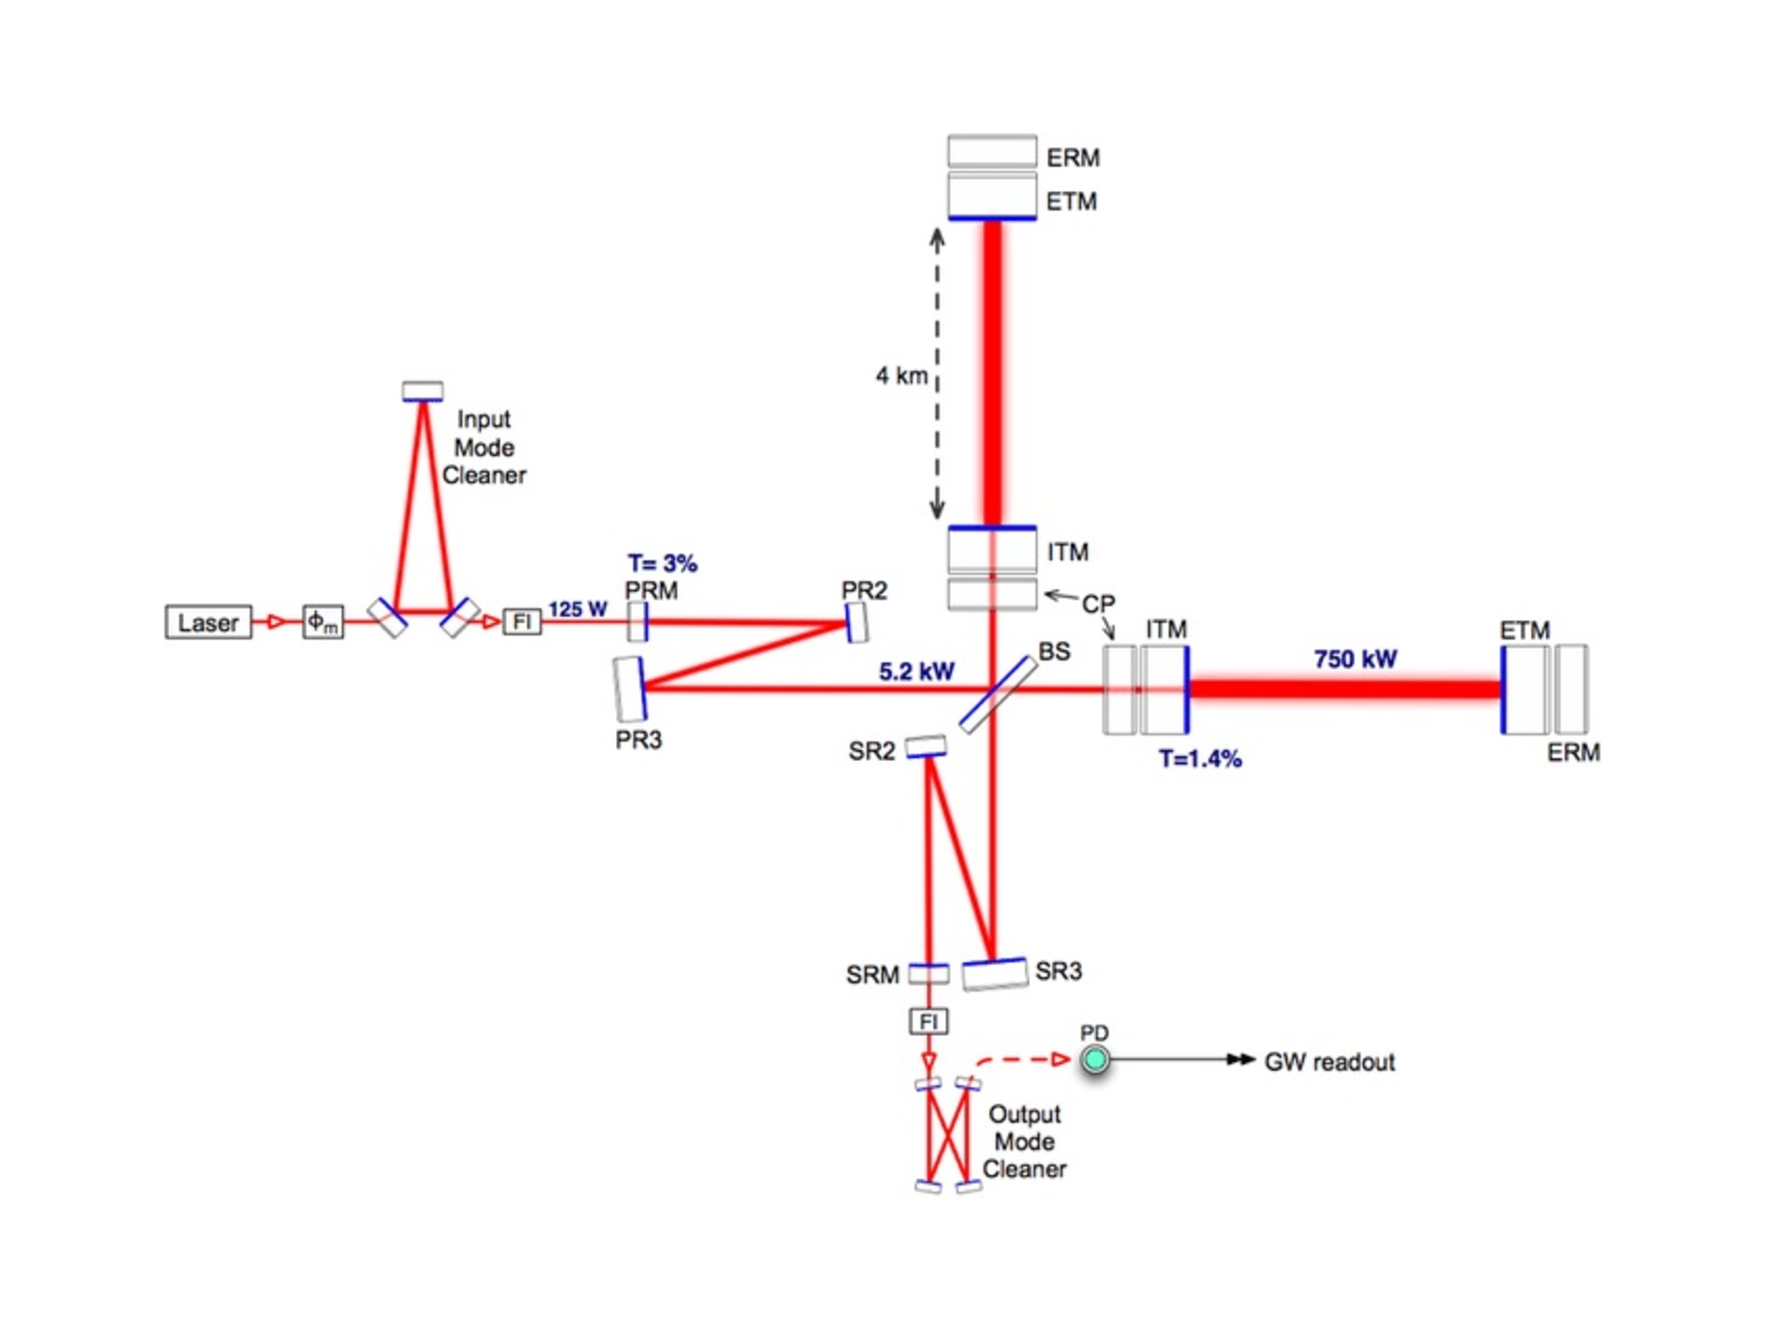
\includegraphics[width=\textwidth]{aligo_config.pdf}
  \end{center}
  \caption{DRFPMI configuration used in ALIGO}
  \label{fig:simple_michelson}
\end{figure}

``Core optics" (Recycling mirrors, Beam splitter, and FP arm cavity mirrors) are suspended with quadruple pendulum suspensions decoupling seismic activity from the mirror positions to as low as a frequency as possible. 

\subsection{Thermodynamic considerations}
Discussions prior to now still have yet to discuss most practical considerations required to operate a DRFPMI as a gravitational wave observatory. For the sake of transitioning to the niche body of this work, I provide a brief discussion of select detector features: 1) adaptive optics for high power operation, and 2) the thermodynamics of highly reflective mirror coatings that impose a fundamental limit to gravitational wave interferometer sensitvity. 

%It is also relevant to know that the studies take place at two very different stages of detector comissoning; one is aimed at comissioning current detectors while the other aims at informing an upgrade choice to be made for current and next generation detectors, though both are aimed at increasing gravitational wave detector sensitivity. The current objective at hand is to inform of these essential criteria for interferometer operations as they pertain to this dissertation. More details on setting up the simple Michelson provides on some of the initial requirements; while the second order is establishing the strict conditions of the Fabry-P\'{e}rot cavities.

%\subsubsection{Length Stabilization}
%With LIGO's coupled cavity configuration, maintaining mirror positions is imperative. Techniques such as the ''side-fringe" lock (using a DC photodiode to measure the transmitted, reflected, or circulating power within a linear and slightly off resonance point) \cite{fox:2003} and the Pound-Drever-Hall technique (see \autoref{subsubsec:pdh} ) are used to maintain cavity length stabilization. Stabilizing cavity lengths to configure the detector into a highly sensitive differential arm sensor is a process that is worthwhile understanding with more ample discussions ~\cite{mullavey:2012}.

%So far, we've discussed light and phase fronts without addressing geometric
%constraints when using Gaussian laser light. We consider a general complex
%Gaussian beam mode propogating along the beam axis ($z$) with wavelength
%$\lambda$
%\begin{equation}\label{eq:gaussianbeam}
%E(r) = E_o \frac{\sqrt{[\lambda z_o] / \pi}}{W(z)}e^{-r^2 / W^2(z)} e^{-ikz - ik[r^2 / (2R(z))] + i \zeta}
%\end{equation}
%
%Where $E_o$ is a complex amplitude, $r = \sqrt{x^2 + y^2}$ defines the transverse beam coordinates, $k$ is the wave number, $W(z)$ is the beam width, $R(z)$ is the beam radius of curvature, and $\zeta$ is the Gouy phase.

%Derived from the paraxial approximation of the Helmholtz equation, this field is not the only solution for optical cavities. Alternative higher order mode (HOM) solutions are commonly present and are expressed in terms of two mathematical bases: the Hermite-Gauss and Laguerre-Gauss modes. These HOMs are more often than not power parasites when attempting to only sense displacement Fabry-P\'{e}rot cavities and are a symptom of altered cavity geometry; though a virtue of the lost power is its utility as an error signal for sensing and actuation schemes. This is what is what is accomplished with an alignment sensing and control (ASC) system and a thermal compensation system (TCS) for mode matching actuation.

%%FIGURE: ALIGO Sensor and Actuation schema

%\subsubsection{Alignment sensing and control}

%\begin{figure}[H]
%    \begin{center}
%    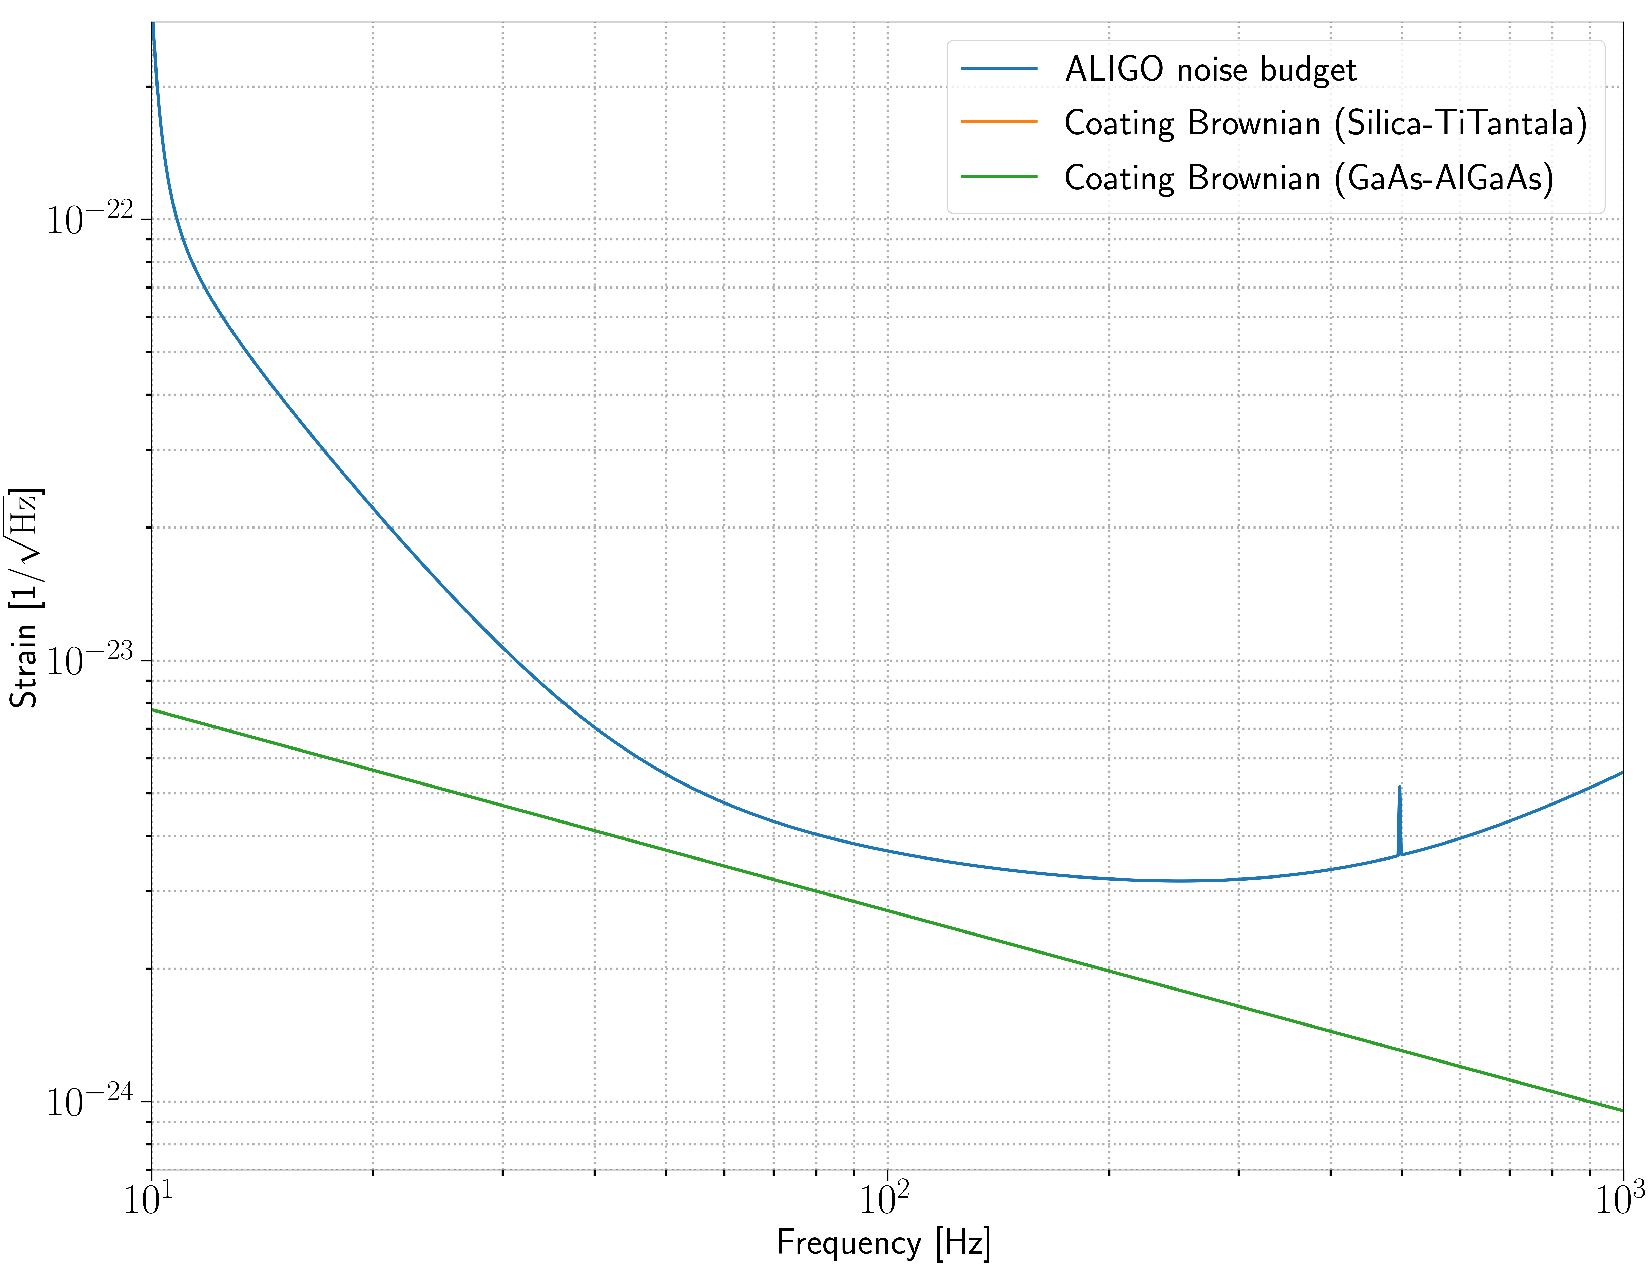
\includegraphics[width=.5\textwidth]{ALGAAS/aligo_nb_plus_cbn.pdf}
%    \end{center}
%    \caption{A misaligned Fabry-P\'{e}rot cavity scatters circulating light into higher order Hermite-Gauss modes.}
%    \label{fig:HGLGmodes}
%\end{figure}

%\textcolor{red}{Cavity misalignment}

%Even with state-of-the-art ground motion isolation for terrestrial gravitational detectors using quadruple stage pendula and high mass mirrors, current gravitational wave detectors still suffer from occasional misalignment and require sensing and feedback loops to meet mirror alignment requirements.

\subsubsection{Adaptive Optics}
As mentioned in \hyperref[subsubsubsubsec:mm2]{\S \ref*{subsubsubsubsec:mm2}} , the microscopic longitudinal control of the mirror positions is only half the story for Gaussian beams and further consideration of macroscopic mirror position and radii of curvature are needed to maximize resonant power in the fundamental (TEM00) mode. Failure to plan and maintain this ``mode matching" condition results in beam mode to cavity mode mismatch, scattering power into higher order Laguerre-Gauss modes. Additionally, even with ultra-low absorption HR mirror coatings and fused silica substrates, aLIGO circulating power is estimated to reach $\geq$ 750 kW, introducing a differential defocus to the arm cavities by [$\mathrm{m}^{-1}$]; which can introduce significant optical loss due to mode mismatch (esp. for a coupled cavity configuration) ~\cite{tvo}. As DRFPMIs like aLIGO approach designed sensitivity, instances of mode mismatch are a two-fold threat with optical loss to higher order modes that impact the ability to produce squeezed light states ~\cite{oelker:2014}. The further motivation and the implemented solution for aLIGO during O3a is discussed in Chapter 2. 

\subsubsection{Coating Thermal Noise}\label{subsubsec:introctn}
Generally speaking, sensed differential arm motion is more often than not produced by sources that are not gravitational waves. The sum and categorization of motion from non gravitational wave sources (both known and unknown) at a given point in time form what is known as a DARM noise budget. This tool aids comissioners in understanding the current limits of GWDs and additionally facilitates focused hypotheses for detector improvements / upgrades. One rapidly approaching limit is the coating thermal noise from the HR $\siotao$ Fabry-P\'erot cavity mirror coatings which arises from the mirror surface position observable influenced by energy dissipated by the coating by way of its acoustic degrees of freedom and causing uncoorelated phase fluctuations between the two arm cavities. Part of the upgrade discussions for current and future GWDs are HR coating materials with different material composition solely for the purpose of lowering this coating thermal noise. A promising candidate with 5 times lower thermal noise properties is the HR crystalline $\gaas/\algaas$ stack. This alone motivates an inquiry into more of its properties, one of which is thoroughly discussed in Chapter 3.   

\begin{figure}[ht!]
    \centering
    \begin{subcaptiongroup}
		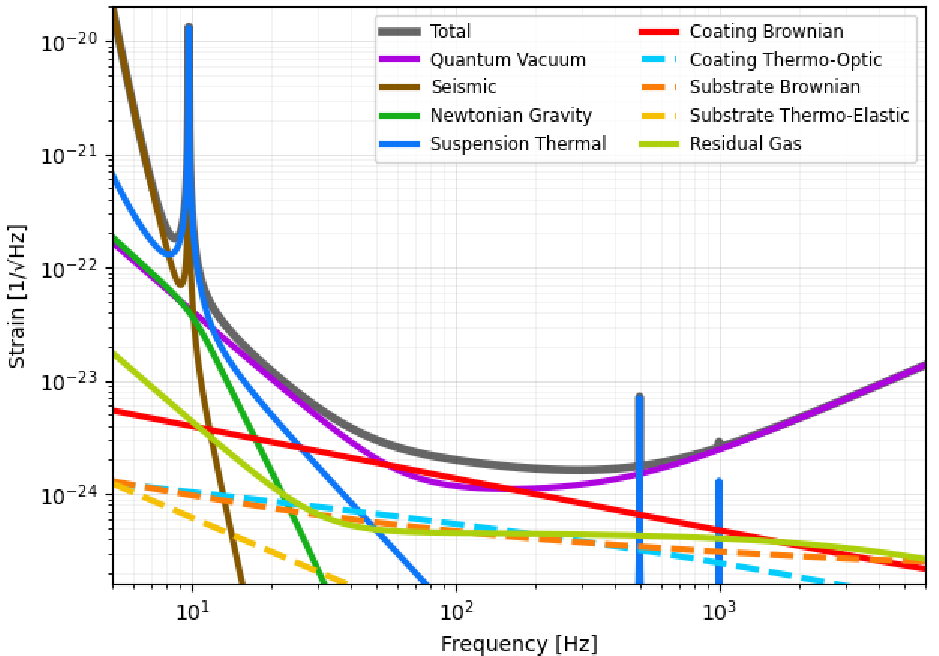
\includegraphics[width=.875\textwidth]{INTRO/Aplus_nb.pdf}
		\\
		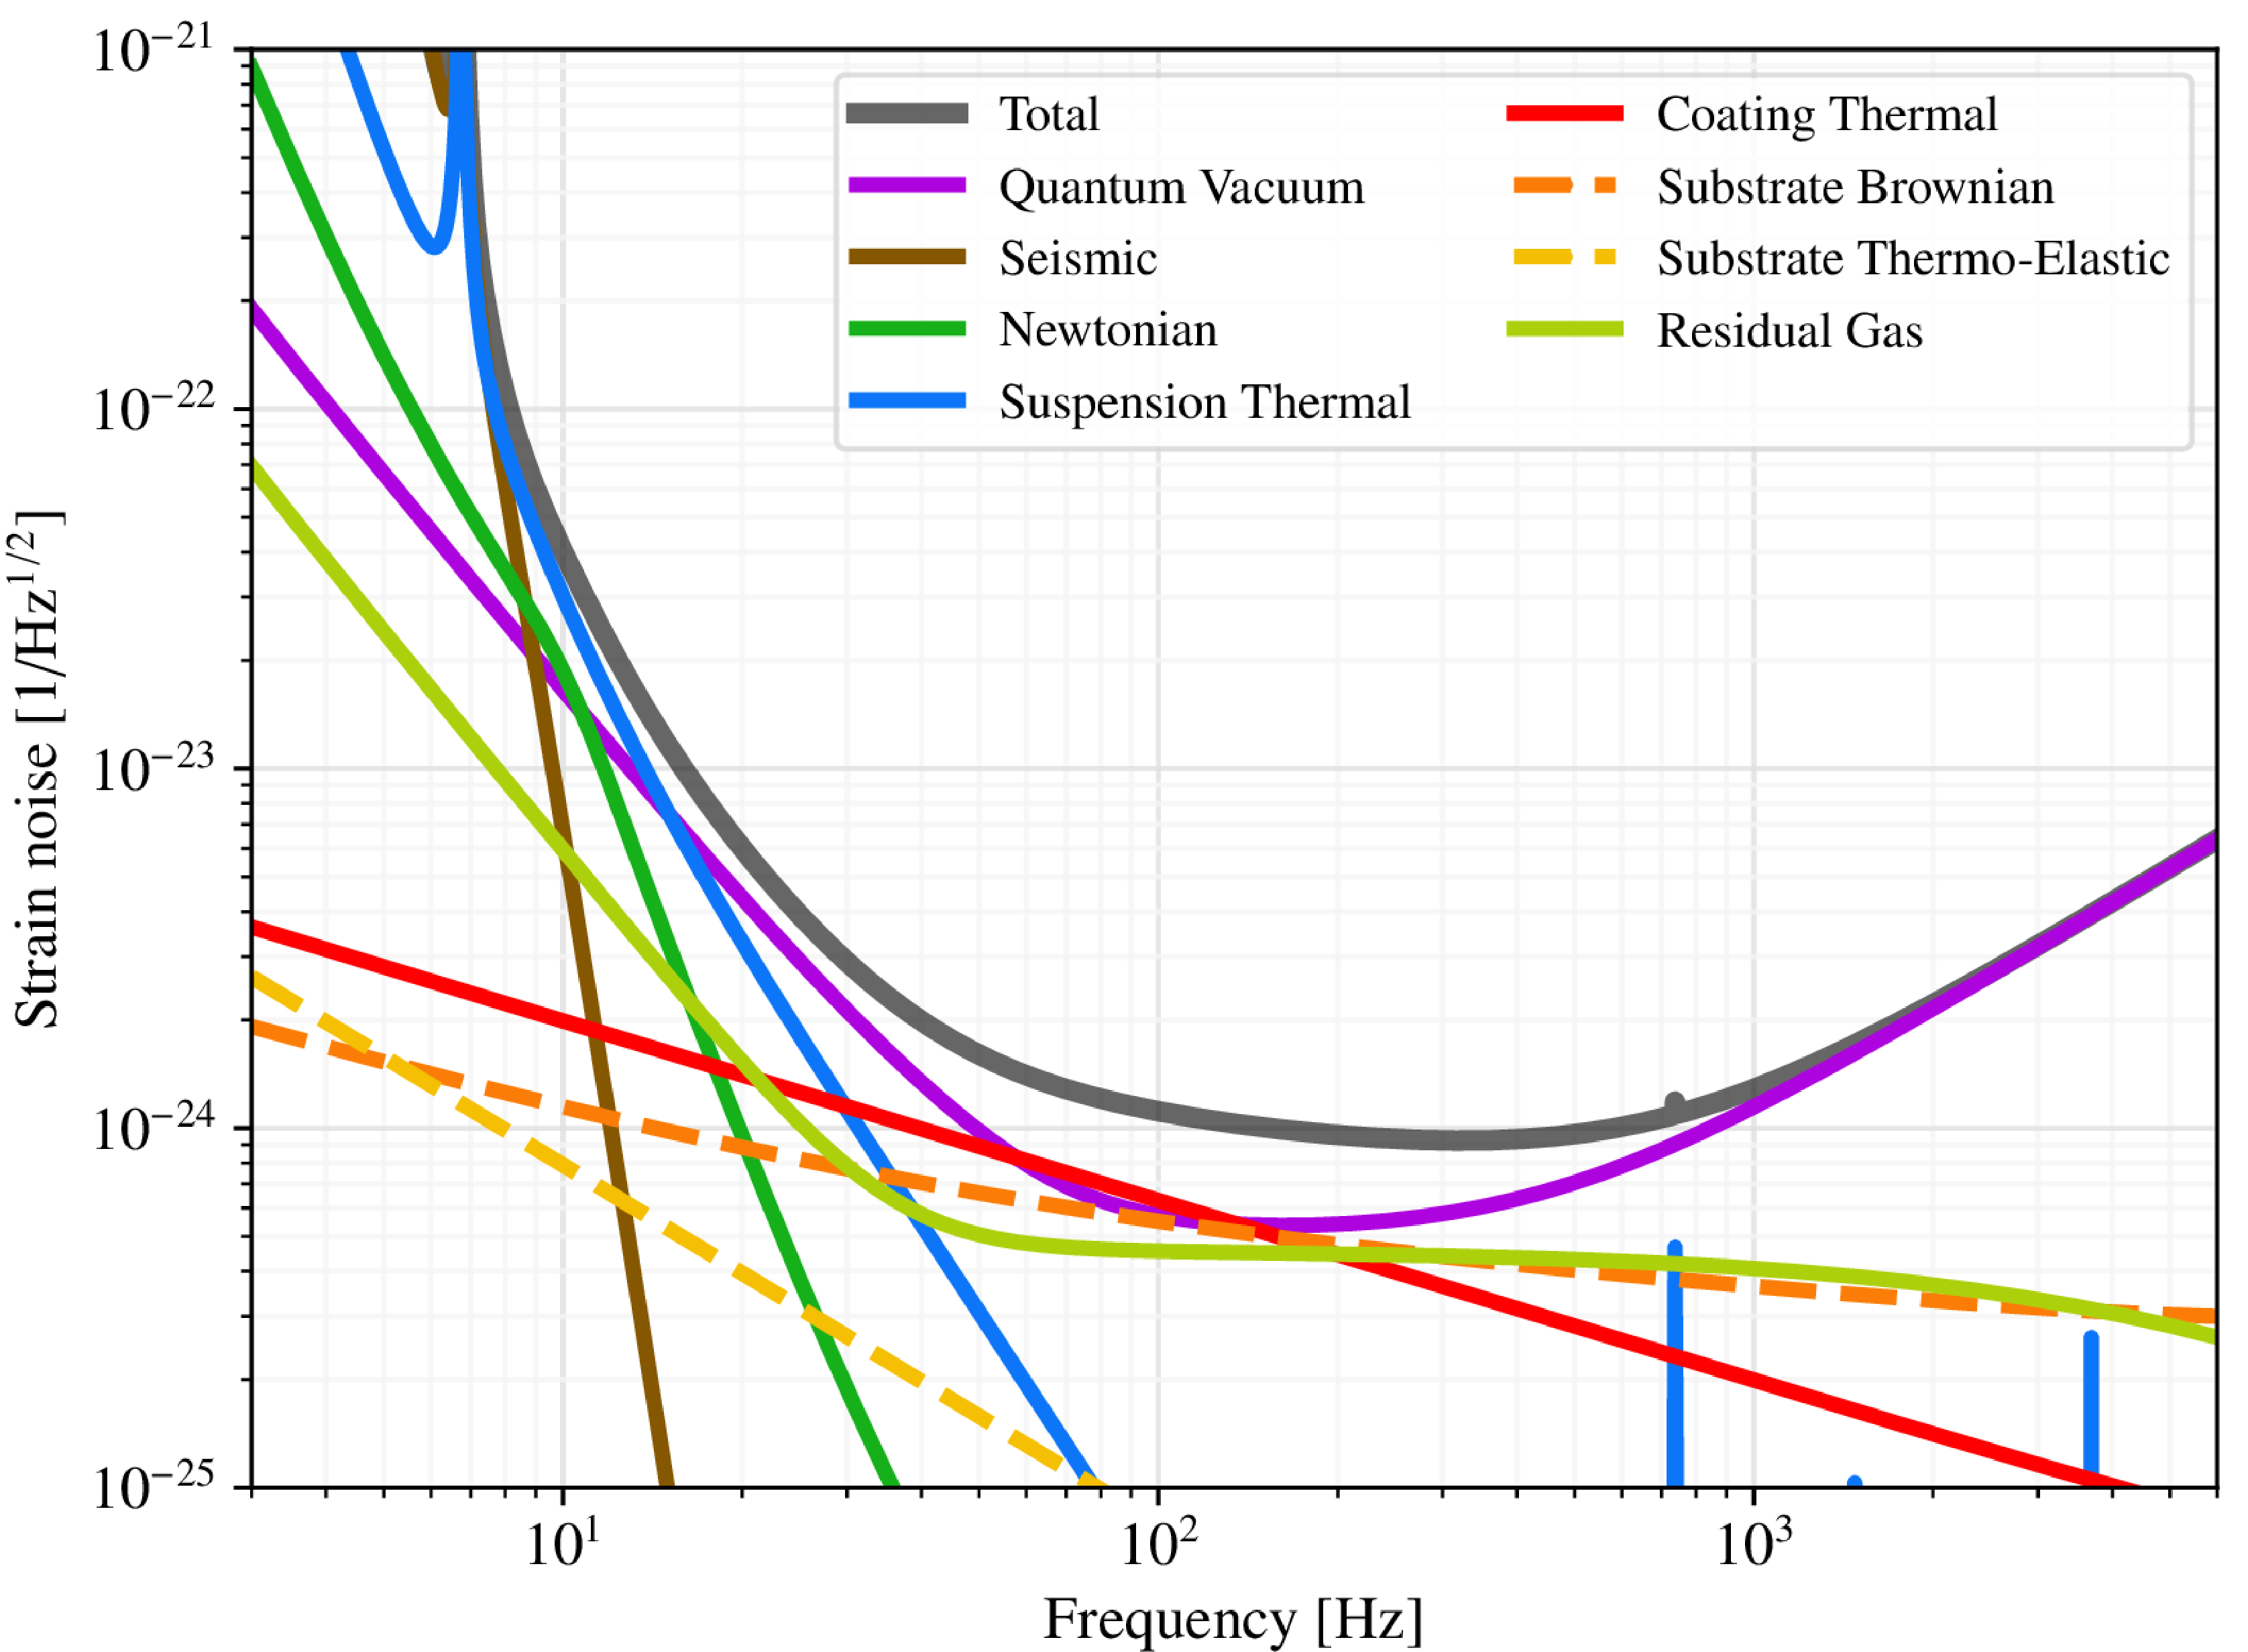
\includegraphics[width=.875\textwidth]{INTRO/Asharp_nb.pdf}
    \end{subcaptiongroup}
    \hfill
    \caption{[Top] Noise budget for the next generation A+ interferometer using $\siotao$ coatings [Bottom] Noise budget for a parallel next generation A$^\sharp$ interferometer using $\gaas$/$\algaas$ coatings~\cite{dcc:asharp}.}
\label{fig:aplusasharp}
\end{figure}


